

%*** General probabilistic notation ***

\newcommand{\expv}{\mathbf{E}} % EXP. VALUE
\newcommand{\discProbDist}{f} % Discrete prob distribution
\newcommand{\sampleSpace}{S} % Generic sample space
\newcommand{\sigmaAlg}{\mathcal{F}} % Generic sigma-algebra
\newcommand{\probm}{\mathbb{P}} % Generic probability measure, also prob. measure operator
\newcommand{\rvar}{X} % Generic random variable
%\newcommand{\dist}{\mathit{Dist}}

%*** MDP notation ***

\newcommand{\actions}{A} % The set of actions.
\newcommand{\colouring}{c} % the colouring function
\newcommand{\probTranFunc}{\Delta} % Transition function of an MDP
\newcommand{\edges}{E} % Set of edges in an MDP.
\newcommand{\colours}{C} % The set of colours in an MDP.
\newcommand{\mdp}{\mathcal{M}} % A generic MDP. 
\newcommand{\vinit}{v_0} % An initial vertex in an MDP.
\newcommand{\cylProb}{p} % Function assigning probabilities to cylinder sets in 
%the measure construction.
\newcommand{\emptyPlay}{\epsilon} %empty play
\newcommand{\objective}{\Omega} % Qualitative objective
\newcommand{\genColour}{\textsc{c}} % Generic colour
\newcommand{\quantObj}{f} % Generic quantitative objective
\newcommand{\indicator}[1]{\mathbf{1}_{#1}} % In.d RV
\newcommand{\eps}{\varepsilon} % Numerical epsilon
\newcommand{\maxc}{W} % Maximal abs. value of a colour

\newcommand{\winPos}{W_{>0}}
\newcommand{\winAS}{W_{=1}}
\newcommand{\cylinder}{\mathit{Cyl}}

\newcommand{\PrePos}{\text{Pre}_{>0}}
\newcommand{\PreAS}{\text{Pre}_{=1}}

\newcommand{\PreOPPos}{\mathcal{P}_{>0}}
\newcommand{\OPAS}{\mathcal{P}_{=1}}

\newcommand{\safeOP}{\mathit{Safe_{=1}}}
\newcommand{\closed}{\mathit{Cl}}

\newcommand{\reachOP}{\mathcal{V}}
\newcommand{\discOP}{\mathcal{D}}
\newcommand{\valsigma}{\vec{x}^{\sigma}}

\newcommand{\lp}{\mathcal{L}}
\newcommand{\lpdisc}{\lp_{\mathit{disc}}}
\newcommand{\lpmp}{\lp_{\mathit{mp}}}
\newcommand{\lpsol}[1]{\bar{#1}}
\newcommand{\lpmpdual}{\lpmp^{\mathit{dual}}}

\newcommand{\actevent}[3]{\actions^{#1}_{#2,#3}} % Returns #1-th action on the run 

\newcommand{\MeanPayoffSup}{\MeanPayoff^{+}}
\newcommand{\MeanPayoffInf}{\MeanPayoff^{-}}

\newcommand{\mcprob}{M}
\newcommand{\invdist}{\vec{z}}

\newcommand{\hittime}{T}



In this chapter, we introduce and review results on stochastic games
with two players. On the one hand, they extend 2-player games with
random vertices; on the other hand, they extend Markov decision
processes with a second player. 

When equipped with a simple reachability objective, the objective of
\Eve is to maximize the probability of the set of plays that reach the
target, while here opponent has the opposite objective. Such games are
positionally determined: optimal positional pure strategies exist (see
Section~\ref{6-sec:values}). Perhaps surprisingly, stochastic games
with reachability objectives are central, in the sense that many more
complex objectives (discounted payoff, mean-payoff, parity) reduce to
them (see Section~\ref{6-sec:relations}). We therefore review several
algorithms to solve stochastic reachability games, based on the value
iteration or strategy improvement principles (see
Section~\ref{6-sec:algos}) that are also used for other classes of
games.



\section*{Notations}
Let us first define the arenas stochastic games will be played on:
\begin{definition}
  A ""stochastic arena"" is a tuple $\arena = (\vertices,E,\delta)$ where
  \begin{itemize}
  \item $\vertices = \VA \sqcup \VE \sqcup \Randomvertices$ is a
    finite set of vertices, partitionned into vertices of \Adam, \Eve,
    and ""random vertices"";
  \item $E \subseteq \vertices \times \vertices$ is the set of
    edges;
  \item $\delta : \Randomvertices \to \dist(\vertices)$ is the
    probabilistic transition function, which satisfies:
    $\forall v \in \Randomvertices$, $\delta(v)(w)>0$ iff
    $(v,w) \in E$.
  \end{itemize}
\end{definition}

\begin{figure}
\centering
    \begin{tikzpicture}[scale=1.3]
    \node[s-eve] (init) at (0,0) {$v_0$};
    \node[s-random] (v1) at (2,0) {$v_1$};
    \node[s-eve] (v2) at (4,0) {$v_2$};    
    \node[s-random] (v3) at (6,0) {$v_3$};
    \node[s-random] (v4) at (0,-1.5) {$v_4$};
    \node[s-eve] (v5) at (2,-1.5) {$v_5$};
    \node[s-adam] (v6) at (4,-1.5) {$v_6$};    
    \node[s-eve] (v7) at (6,-1.5) {$v_7$};
    
    \path[arrow] (init) edge (v1)
    (init) edge[bend left] (v4)
    (v4) edge[bend left] node[left] {$\frac 3 4$} (init)
    (v4) edge node[above] {$\frac 1 4$} (v5)
    (v5) edge[bend left] (v6)
    (v6) edge (v7)
    (v6) edge[bend left] (v5)
    (v5) edge[selfloop=90]  (v5)
    (v7) edge[selfloop]  (v7)
    (v1) edge node[above] {$\frac 2 3$} (v2)
    (v1) edge node[above right] {$\frac 1 3$} (v6)
    (v2) edge (v6)
    (v2) edge[bend left] (v3)
    (v3) edge[bend left] node[below] {$\frac 1 2$} (v2)
    (v3) edge node[right] {$\frac 1 2$} (v7)
%    (init) edge node[left] {$\frac 1 {10}$} (av)
%    (init) edge node[left] {$\frac 3 {10}$} (rv)
%    (init) edge node[right] {$\frac 2 {5}$} (ev)
    ;    
% \node[s-random] (root) at (0,0) {$v$};
% \node[s-random] (left) at (-.75,-1) {};
% \node[s-random] (right) at (.75,-1) {};
% \node[s-adam] (lleft) at (-1.5,-2) {$v_1$};
% \node[s-random] (rleft) at (0,-2) {$v_2$};
% \node[s-eve] (rright) at (.75,-2) {$v_3$};

% \path[arrow] (root) edge node[left] {$\frac 2 5$}  (left)
% (root) edge node[right] {$\frac 3 5$}  (right)
% (left) edge node[left] {$\frac 1 4$} (lleft)
% (left) edge node[right] {$\frac 3 4$} (rleft)
% (right) edge node[right] {$\frac 2 3$} (rright)
% (right) edge[out=70,in=0] node[right] {$\frac 1 3$} (root)
% % (ab) edge [loop] (ab)
% % (notb) edge  node [above] {} (notab)
% % (notab) edge   (ab)
% % (ab) edge[out=195,in=-15] (notab)
% % (ab) edge[out=205,in=-25] (notb)
% ;
    \end{tikzpicture}
  \caption{Example of a stochastic arena: circle nodes belong to \Eve,
    square nodes to \Adam, and diamond nodes are random.}
  \label{6-fig:ex-stoch-arena}
\end{figure}


Similarly to non-stochastic arenas, one can equip a stochastic arena
with a winning objectives to define a stochastic game.
\begin{definition}
  A ""stochastic game"" is a tuple $\game = (\arena,\Omega)$ where
  \begin{itemize}
  \item $\arena$ is a stochastic arena;
  \item $\Omega \subseteq \vertices^\omega$ is the (qualitative)
    winning objective.
  \end{itemize}
\end{definition}

For $\Win \subseteq \vertices$, letting $\Omega = \Reach(\Win)$ gives
rise to a stochastic reachability game.
Of course, one may consider more general $\omega$-regular
properties. We write $\mathds{1}_\Omega$ for the characteristic
function of the winning objective $\Omega$.


In this game, \Eve aims at maximizing the probability that a play
belongs to $\Omega$, while \Adam has the opposite objective of
minimizing that probability. In that sense, we study quantitative
games, although the winning objective is qualitative.

A \emph{strategy} for \Eve is a function
$\sigma: V^* \VE \to \dist(\vertices)$ such that whenever
$\sigma(h v)(v') >0$ then $(v,v') \in E$. Similarly, one can define
strategies for \Adam. When a strategy profile $(\sigma,\tau)$ is
fixed, and assuming the arena is clear from context, we write
$\probm_{\sigma,\tau}^v$ for the probability measure on infinite plays
when the initial vertex is $v$. In particular,
$\probm_{\sigma,\tau}^v(\mathds{1}_\Omega)$ is the outcome of the profile
$(\sigma,\tau)$.


% We note $\probm_{\sigma,\tau}^v$ without the name of the game when it
% is evident.
% We will also write $\sigma(h)(\adist,v')$ 

% \textit{Strategies}
% $\sigma$: strategies of \Eve; $\tau$: strategies of \Adam

%\textit{Notions  of inf value, sup value}

The \emph{"value" for \Eve} in $\game$ from $v$ is defined as
$\ValueE^\game(v) = \sup_{\sigma} \inf_{\tau}
\probm_{\sigma,\tau}^v(\mathds{1}_\Omega)$, whereas symmetrically the
\emph{supremum value} is
$\ValueA^\game(v) = \inf_{\tau}\sup_{\sigma}
\probm_{\sigma,\tau}^v(\mathds{1}_\Omega)$. Clearly enough,
$\ValueE^\game(v) \leq \ValueA^\game(v)$.  When the converse
inequality holds, the game is \emph{determined} and the \emph{value}
of $v$ in $\game$ is denoted $\Value^\game(v)$. Moreover, if the value
is attained by positional strategies $\sigma$ and $\tau$, $\game$ is
said to be \emph{positionally determined}. \emph{Strong determinacy}
means that for every threshold $c$, either \Eve has a strategy to
ensure that the probability that the play belongs to $\Omega$ is at
least $c$, or \Adam has a strategy to ensure probability $< c$ to for
the set of plays satisfying $\Omega$.

Back to the example of Figure~\ref{6-fig:ex-stoch-arena}, assume that
\Eve and \Adam play the following pure positional strategies:
$\sigma(v_0) = v_1$, $\sigma(v_2) = v_3$, $\sigma(v_5) = v_5$ and
$\tau(v_6) = v_5$. Under such a strategy profile, starting in $v_0$,
the probability to reach $v_7$ is
$\probm_{\sigma,\tau}^{v_0}(\mathds{1}_{\Reach(\{v_7\})}) = \frac 2
3$. In fact, strategy $\sigma$ for \Eve is optimal for the
reachability objective $\Reach(\{v_7\})$, and we will justify that
$\ValueE^\game(v_0) = \ValueA^\game(v_0) = \frac 2 3$.



\section{Positional determinacy of stochastic reachability games}
\label{6-sec:values}
\label{6-sec:determinacy}
% \begin{itemize}
% \item discussion qualitative vs quantitative: qualitative is a rather
%   small extension of non-stochastic games. We only need to encode
%   fairness into the winning condition, which is not too difficult
%   using a parity condition. Hence we will mostly focus on the
%   quantitative question.
% \item Speak of qualitative and quantitative determinacy
% \end{itemize}


% \fbox{parler de la quantitative determinacy des Blackwell games
%   [Mar98] ?}
Pure memoryless determinacy for non-stochastic games with parity
objectives was established in~\cref{2-chap:regular} (see~\cref{2-thm:parity}). 
In this section we extend this result to stochastic games. 
We focus on reachability objectives, since we will see in~\cref{6-sec:relations} 
that other natural objectives reduce to reachability.

%\fbox{check whether pure memoryless determinacy is preserved by
%  these reductions}

\begin{theorem}[Pure positional determinacy for stochastic reachability games]
\label{6-thm:determinacy}
Stochastic reachability games are pure positionally determined.
\end{theorem}

\begin{proof}
  Let $G = (\vertices,E,\delta,\Win)$ be a stochastic reachability
  game.  We define an operator $\mathfrak{F}$ expressing Bellman-like
  equations for the game $G$:
  \[
  \mathfrak{F}(\nu)(v) = \left\{\begin{array}{l@{~~}l}
      1 & \text{if}\ v = \Win \\
      \max_{(v,v') \in E} \nu(v') & \text{if}\ v \in \VE \\
      \min_{(v,v') \in E} \nu(v') & \text{if}\ v \in \VA \\
      \sum_{v' \in \vertices} \delta(v)(v') \cdot \nu(v') & \text{if} \in \Randomvertices
    \end{array}\right.
  \]
  This operator, defined on the complete lattice $[0,1]^{\vertices}$
  (equipped with the pointwise standard inequality) is
  monotonic. Hence it admits a least fixpoint, which we denote
  $\lfp(\mathfrak{F})$.  We show that:
  \begin{lemma}
    \label{6-lem:lfpgeval}
    For every $v$:
    \[
    \lfp(\mathfrak{F}) (v) \le \sup_\sigma \inf_\tau
    \probm_{\sigma,\tau}^v(\Reach(\Win)) \le \inf_\tau \sup_\sigma
    \probm_{\sigma,\tau}^v(\Reach(\Win)) \enspace.
    \]
  \end{lemma}
  \begin{proof}
    We first argue for the right inequality:
    \begin{eqnarray*}
      \forall \sigma' \forall \tau:\
      \probm_{\sigma',\tau}^v(\Reach(\Win)) & \le & \sup_\sigma
      \probm_{\sigma,\tau}^v(\Reach(\Win)) \\
      \forall \sigma'\forall \tau :\  \inf_{\tau'}
      \probm_{\sigma',\tau'}^v(\Reach(\Win)) & \le & \sup_\sigma
      \probm_{\sigma,\tau}^v(\Reach(\Win)) \\
      \forall \tau:\ \sup_{\sigma'} \inf_{\tau'}
      \probm_{\sigma',\tau'}^v(\Reach(\Win)) & \le & \sup_\sigma
      \probm_{\sigma,\tau}^v(\Reach(\Win)) \\
      \sup_{\sigma'} \inf_{\tau'}
      \probm_{\sigma',\tau}'^v(\Reach(\Win)) & \le & \inf_{\tau} \sup_\sigma
      \probm_{\sigma,\tau}^v(\Reach(\Win)) 
    \end{eqnarray*}

    For proving the left inequality, it is sufficient to show that
    $v \mapsto \sup_\sigma \inf_\tau
    \probm_{\sigma,\tau}^v(\Reach(\Win))$ is a fixpoint of
    $\mathfrak{F}$.  Pick $v \in \VE$. 
    % First, when $\sigma$ and $\tau$
    % are both fixed, then
    % \[
    %   \probm_{\sigma,\tau}^v(\Reach(\Win)) = \sum_{v' \in
    %     \text{supp}(\sigma(v))} \sigma(v)(v') \cdot
    %   \probm_{\sigma'_{v'},\tau'}^{v'}(\Reach(\Win))
    % \]
    % where, given $v' \in \text{supp}(\sigma(v))$, $\sigma'_{v'}$ is
    % the strategy coinciding with $\sigma$ after the first move to $v'$
    % (formally, $\sigma'_{v'}(v' h) = \sigma(v v' h)$ for every finite
    % sequence of vertices $h$).
 \begin{eqnarray*}
      \sup_\sigma \inf_\tau \probm_{\sigma,\tau}^v(\Reach(\Win)) & = &
      \sup_\sigma \inf_\tau \sum_{v'} \sigma(v)(v')  \cdot
      \probm_{\sigma',\tau'}^{v'}(\Reach(\Win)) \\
      & & \text{where}\ \sigma'\ \text{and}\ \tau'\ \text{are residual
        strategies after}\ (v,v') \\
      & = & \sup_\sigma \sum_{v'} \sigma(v)(v')  \cdot \inf_\tau \probm_{\sigma',\tau'}^{v'}(\Reach(\Win)) \\
      & & \text{since}\ \tau\ \text{is not concerned by this choice}
      \\
      & = & \max_{(v,v') \in E} \sup_{\sigma\ \text{s.t.}\
        \sigma(v) = v'} \inf_\tau
      \probm_{\sigma',\tau'}^{v'}(\Reach(\Win)) \\
      & & \text{since deterministic choices are the best} \\
      & = & \max_{(v,v') \in E} \sup_{\sigma'} \inf_{\tau'}
      \probm_{\sigma',\tau'}^{v'}(\Reach(\Win)) \\
      & & \text{since the first choice is now fixed} \\
      & = & \mathfrak{F}(\probm_{\sigma,\tau}^{\bullet}(\Reach(\Win)))(v)
    \end{eqnarray*}
    where $\probm_{\sigma,\tau}^{\bullet}(\Reach(\Win)))$ is the
    function with associates with vertex $v$ the value
    $\probm_{\sigma,\tau}^{v}(\Reach(\Win)))$.
    % \begin{eqnarray*}
    %   \sup_\sigma \inf_\tau \probm_{\sigma,\tau}^v(\Reach(\Win)) & = &
    %   \sup_\sigma \inf_\tau \sum_{v'} \sigma(v)(V'd)
    %   \cdot \probm_{\sigma',\tau'}^{v'}(\Reach(\Win)) \\
    %   & & \text{where}\ \sigma'\ \text{and}\ \tau'\ \text{are residual
    %     strategies after}\ (v,\adist,v') \\
    %   & = & \sup_\sigma \sum_{(\adist,v')} \sigma(v)(\adist,v')
    %   \cdot \inf_\tau \probm_{\sigma',\tau'}^{v'}(\Reach(\Win)) \\
    %   & & \text{since}\ \tau\ \text{is not concerned by this choice}
    %   \\
    %   & = & \max_{(v,\adist) \in E} \sup_{\sigma\ \text{s.t.}\
    %     \sigma(v) = \adist} \inf_\tau
    %   \probm_{\sigma',\tau'}^{v'}(\Reach(\Win)) \\
    %   & & \text{since deterministic choices are the best} \\
    %   & = & \max_{(v,\adist) \in E} \sup_{\sigma'} \inf_{\tau'}
    %   \probm_{\sigma',\tau'}^{v'}(\Reach(\Win)) \\
    %   & & \text{since the first choice is now fixed} \\
    %   & = & \mathfrak{F}(\probm_{\sigma,\tau}^{\bullet}(\Reach(\Win)))(v)
    % \end{eqnarray*}

    Assume now that $v \in \VA$. 
    % \begin{eqnarray*}
    %   \sup_\sigma \inf_\tau \probm_{\sigma,\tau}^v(\Reach(\Win)) & = &
    %   \sup_\sigma \inf_\tau \sum_{(\adist,v')} \tau(v)(\adist,v')
    %   \cdot \probm_{\sigma',\tau'}^{v'}(\Reach(\Win)) \\
    %   & & \text{where}\ \sigma'\ \text{and}\ \tau'\ \text{are residual
    %     strategies after}\ (v,\adist,v') \\
    %   & = & \sup_\sigma \min_{(v,\adist) \in E} \inf_{\tau\
    %     \text{s.t.}\ \tau(v) = \adist} \sum_{v'} \tau(v)(\adist,v')
    %   \cdot \probm_{\sigma',\tau'}^{v'}(\Reach(\Win)) \\
    %   & & \text{since deterministic choices are the best} \\
    %   & = & \min_{(v,\adist) \in E}  \sup_{\sigma'} \inf_{\tau\
    %     \text{s.t.}\ \tau(v) = \adist} \sum_{v'} \tau(v)(\adist,v')
    %   \cdot \probm_{\sigma',\tau'}^{v'}(\Reach(\Win)) \\
    %   & & \text{since}\ \sigma\ \text{is not concerned with the first
    %     choice} \\
    %   & = & \mathfrak{F}(\probm_{\sigma,\tau}^{\bullet}(\Reach(\Win)))(v)
    % \end{eqnarray*}
    \begin{eqnarray*}
      \sup_\sigma \inf_\tau \probm_{\sigma,\tau}^v(\Reach(\Win)) & = &
      \sup_\sigma \inf_\tau \sum_{v'} \tau(v)(v')
      \cdot \probm_{\sigma',\tau'}^{v'}(\Reach(\Win)) \\
      & & \text{where}\ \sigma'\ \text{and}\ \tau'\ \text{are residual
        strategies after}\ (v,v') \\
      & = & \sup_\sigma \min_{(v,v') \in E} \inf_{\tau\
        \text{s.t.}\ \tau(v) = v'} 
       \probm_{\sigma',\tau'}^{v'}(\Reach(\Win)) \\
      & & \text{since deterministic choices are the best} \\
      & = & \min_{(v,v') \in E}  \sup_{\sigma'} \inf_{\tau\
        \text{s.t.}\ \tau(v) = v'} \probm_{\sigma',\tau'}^{v'}(\Reach(\Win)) \\
      & & \text{since}\ \sigma\ \text{is not concerned with the first
        choice} \\
      & = & \mathfrak{F}(\probm_{\sigma,\tau}^{\bullet}(\Reach(\Win)))(v)
    \end{eqnarray*}

    Finally, let  $v \in \Randomvertices$. 
    \begin{eqnarray*}
      \sup_\sigma \inf_\tau \probm_{\sigma,\tau}^v(\Reach(\Win)) & = & \sum_{v'} \delta(v)(v') \cdot \sup_{\sigma'} \inf_{\tau'} \probm_{\sigma',\tau'}^{v'}(\Reach(\Win))\\
            & & \text{where}\ \sigma'\ \text{and}\ \tau'\ \text{are residual
                strategies after}\ (v,v') \\
      & = & \mathfrak{F}(\probm_{\sigma,\tau}^{\bullet}(\Reach(\Win)))(v)
    \end{eqnarray*}
    This concludes the proof.
%
    
  \end{proof}

  \begin{lemma}
    \label{6-lem:lfpleval}
    For every $v \in \vertices$:
    \[
    \lfp(\mathfrak{F})(v) \ge \inf_\tau \sup_\sigma
    \probm_{\sigma,\tau}^v(\Reach(\Win)) \enspace.
    \]
  \end{lemma}

  \begin{proof}
    Let $v \in \VA$. Since $\lfp(\mathfrak{F})$ is a fixpoint of
    $\mathfrak{F}$, and because the arena is finitely branching, there exists $v'\in \vertices$ such
    that $(v,v') \in E$ and:
    \[
      \lfp(\mathfrak{F})(v) = \lfp(\mathfrak{F})(v') \enspace.
    \]
    We define $\tau^*$ the MD strategy, that selects for every
    $v\in \VA$ such a vertex $v'$, and we show now that for every
    $v \in \vertices$:
    \[
    \lfp(\mathfrak{F})(v) = \sup_\sigma
    \probm_{\sigma,\tau^*}^v(\Reach(\Win)) \enspace.
    \]
    When $\tau^*$ is fixed, the game becomes a finite Markov decision
    process $\game_{\tau^*}$ (in that MDP, the random vertices are
    isolated from the non-deterministic ones, see
    Remark~\ref{5-rk:??}). Note that by standard results on MDP,
    see~\ref{5-thm:quantireach} there exists $\sigma^*$ MD such that
    for every $v \in V$:
    \[
    \probm_{\sigma^*,\tau^*}^v(\Reach(\Win)) = \sup_\sigma
    \probm_{\sigma,\tau^*}^v(\Reach(\Win)) \enspace.
    \]
    Furthermore, $\probm_{\sigma^*,\tau^*}^\bullet(\Reach(\Win))$ is
    the least fixpoint of the Bellman equations for the MDP
    $\game_{\tau^*}$ (see~\ref{5-eq:Bellman}).
    
    It remains to observe that $\lfp(\mathfrak{F})$ satisfies the
    Bellman equations of the MDP under $\tau^*$: this is true from
    \Eve vertices since equations at those vertices are the same in
    the game and in the MDP; this is true from \Adam vertices by local
    optimality of $\tau^*$. Hence we deduce that
    \[
      \lfp(\mathfrak{F}) \ge
      \probm_{\sigma^*,\tau^*}^\bullet(\Reach(\Win)) = \sup_\sigma
      \probm_{\sigma,\tau^*}^\bullet(\Reach(\Win)) \ge \inf_\tau
      \sup_\sigma \probm_{\sigma,\tau}^\bullet(\Reach(\Win)) \enspace.
    \]
    This concludes the proof of the lemma. 
  \end{proof}
By Lemma~\ref{6-lem:lfpgeval} and~\ref{6-lem:lfpleval}  we derive that:
 \[
   \lfp(\mathfrak{F}) =
   \sup_\sigma \inf_\tau 
    \probm_{\sigma,\tau}^\bullet(\Reach(\Win)) =  \inf_\tau \sup_\sigma
   \probm_{\sigma,\tau}^\bullet(\Reach(\Win)) = 
   \probm_{\sigma^*,\tau^*}^\bullet(\Reach(\Win)) \enspace.
  \]
  This proves that $\game$ is pure memoryless determined, and that
  $(\sigma^*,\tau^*)$ is an optimal pure positional strategy profile.
  % \begin{itemize}
  % \item $\tau^*$ is optimal (and MD)
  % \item $\sigma^*$ is optimal (and MD)
  % \item we can compute the values by iterating $\mathfrak{F}$ 
  % \end{itemize}
  %
   
\end{proof}

The proof of Theorem~\ref{6-thm:determinacy} yields an algorithm to
compute the value of a stochastic game with reachability
objective. Indeed, because the value in every vertex $v \in \vertices$
agrees with $\lfp(\mathfrak{F})(v)$, it suffices to compute
iteratively approximations of the fixpoint $\lfp(\mathfrak{F})$.  This
provides the first value iteration algorithm for general stochastic
reachability games.

Historically this result was proven in the restricted framework of
stopping games. The stochastic game $\game = (\arena,\Omega)$ is said
stopping whenever the arena $\arena$ has two distinguished sink
vertices $\vwin$ and $\vlose$, and for all strategies $\sigma$ and
$\tau$, for every vertex $v$,
$\probm_{\sigma,\tau}^{\arena,v}(\Reach(\{\vwin,\vlose\})) =
1$. Whenever the game is stopping, $\mathfrak{F}$ has a unique
fixpoint, hence the value iteration algorithm can be applied from any
initial tuple of values.
% \fbox{say more?}  Originally papers assume stopping games...

% \nat{The positional determinacy also holds for stochastic parity games
%   (see CHJ-soda04). Check whether it is a byproduct of reductions.}

% \begin{remark}
%   Let $\arena$ be an arena with two distinguished sink vertices
%   $\vwin$ and $\vlose$. Assume $\Omega$ is the reachability objective
%   $\Reach(\Win)$ where $\Win = \{\vwin\}$. The stochastic game $\game
%   = (\arena,\Omega)$ is said stopping whenever for all strategies
%   $\sigma$ and $\tau$,
%   $\probm_{\sigma,\tau}^{\arena,v}(\Reach(\{\vwin,\vlose\})) = 1$ for
%   every vertex $v$. Whenever the arena/game is stopping,
%   $\mathfrak{F}$ has a unique fixpoint. \fbox{say more?}
% \end{remark}

Notice that the proof of Theorem~\ref{6-thm:determinacy} and the value
iteration algorithm which derives from it do not assume that the game
is stopping, nor that distributions are uniform.


\section{Relations between all games}
\label{6-sec:relations}
Stochastic reachability games are powerful enough to encode
non-stochastic discounted games. 
More interestingly, they are central to the analysis of several important classes of stochastic
games: in particular, stochastic games with parity objectives,
mean-payoff objectives or discounted payoff all reduce to stochastic
reachability games. This motivates the fact that we focused on
reachability for determinacy in~\Cref{6-sec:determinacy}), and that
in~\Cref{6-sec:algos} we only give algorithms for stochastic games
with reachability objectives.


% A schema with the links between non-stochastic MP-discounted-parity
% games and stochastic MP-discounted-parity games, and SSGs.
% 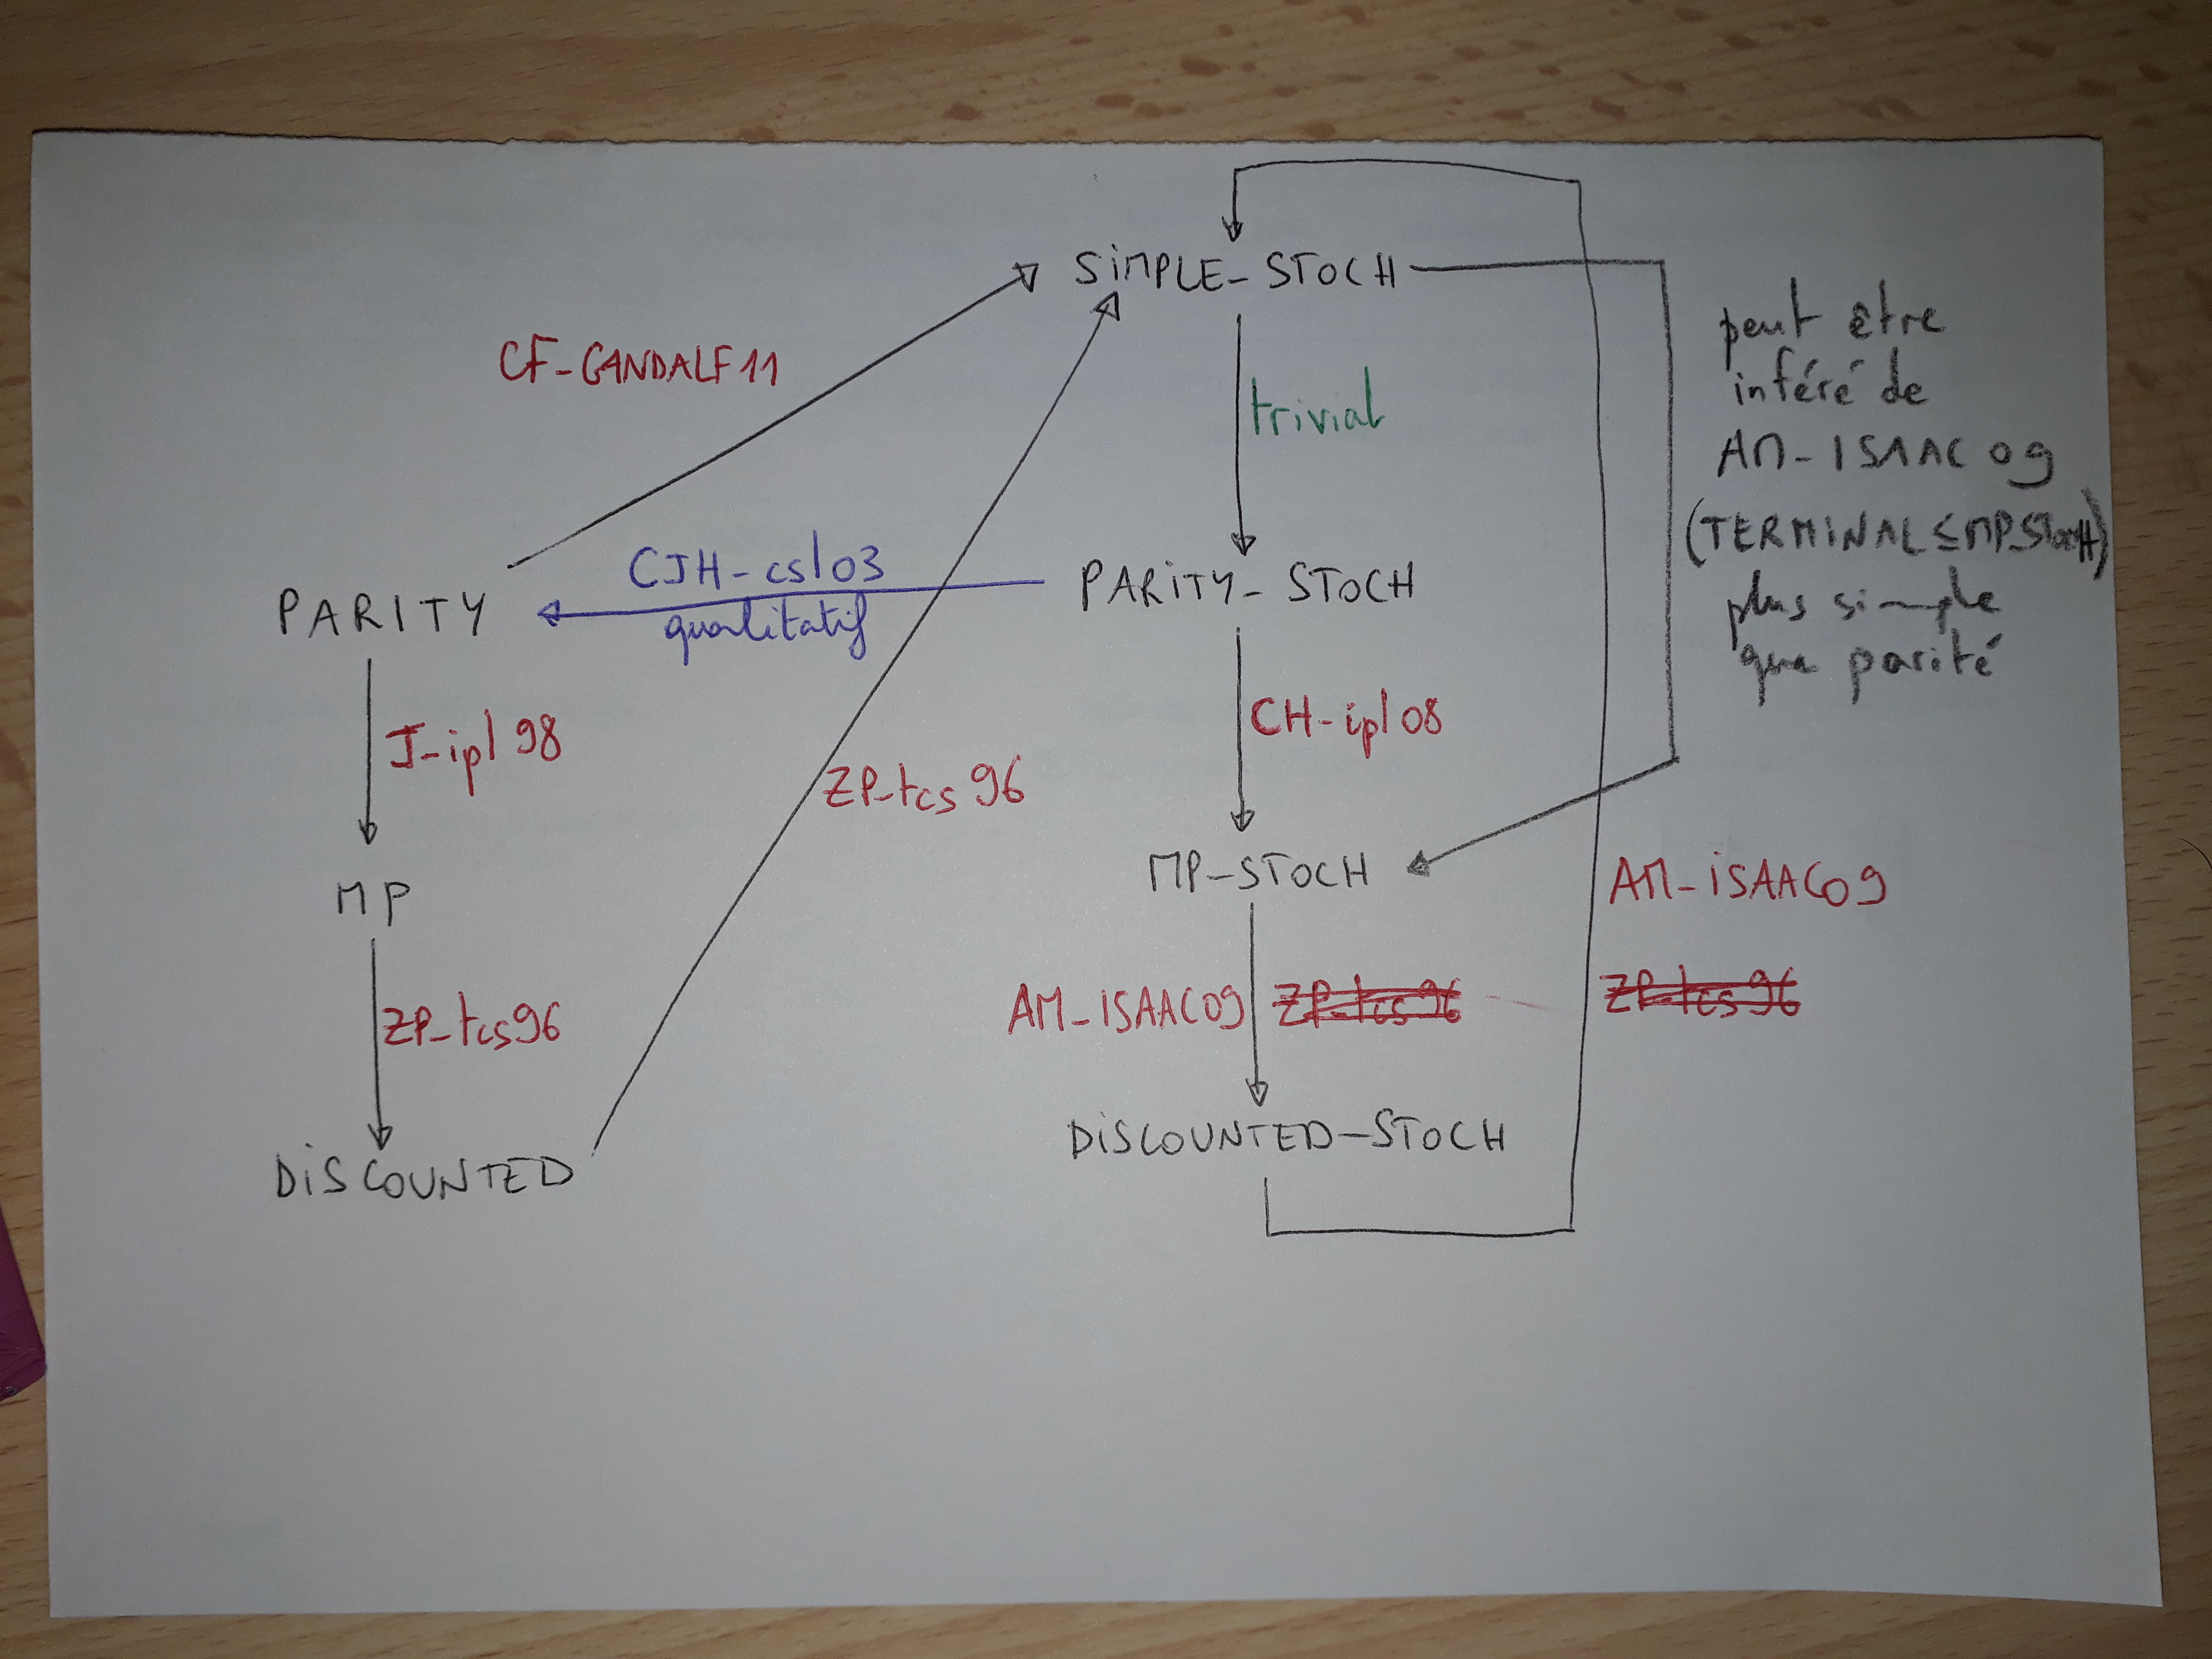
\includegraphics[width=\textwidth]{schema-SSG.jpg}


\subsection{From discounted games to stochastic reachability games}
\nat{reference: ZP-tcs96}

\begin{proposition}
  \label{prop:dg2ssg}
  For any arena $\arena$ with weights in $[0,1]$ and $\lambda$ a
  discount factor, one can construct a stochastic arena $\arena'$ with
  $\Win \subseteq \vertices'$ and an injection
  $\iota : \vertices \to \vertices'$ such that
  $\forall v \in \vertices$
  \[
    \mathsf{value}(v,\arena,\textrm{discount}(\lambda)) =
    \mathsf{value}(\iota(v),\arena',\Reach(\Win)) \enspace.
  \]
\end{proposition}

\begin{proof}
  The idea of the transformation is simple. The vertices in $\arena'$
  are formed of the vertices in $\arena$ plus two sink vertices
  $\smiley$ and $\frownie$, and some fresh random vertices. Then, an
  edge $e = (v,\weight,v')$ of $\arena$ is simulated in $\arena'$ with
  a transition from $v$ to a random vertex $v_e$, and the distribution
  $\delta(v_e)$ assigns probability $\lambda$ to $v'$,
  $(1{-}\lambda)\weight$ to $\smiley$ and $(1{-}\lambda)(1{-}\weight)$
  to $\frownie$. The set $\Win$ of target vertices in $\arena'$
  consists of $\{smiley\}$. To complete the reduction, we let $\iota$
  be the identity function on vertices of $\arena$.

  Note that the transformation from $\arena$ to $\arena'$ is clearly
  polynomial.


  To establish that this transformation preserves the values,
  \emph{i.e.}\ that for every $v \in \vertices$,
  $\mathsf{value}(v,\arena,\textrm{discount}(\lambda)) =
  \mathsf{value}(v,\arena',\Reach(\Win))$, we prove that these
  values are solutions to the same system of equations.

  In the sequel, we write $\mathsf{value}_{\arena'}(v)$ as a shortcut
  for $\mathsf{value}(v,\arena',\Reach(\Win))$.
  By~\Cref{th:determinacy}, the values in the stochastic simple game
  $\arena'$ are solutions to the system of Bellman equations. The sink
  vertices have trivial values, $\mathsf{value}_{\arena'}(\smiley) =1$
  and $\mathsf{value}_{\arena'}(\frownie) =0$.  For every non-random
  vertex $v \notin \{\smiley,\frownie\}$ in $\arena'$,
  \[
    \mathsf{value}_{\arena'}(v)
  = \begin{cases}   \max_{(v,v_e) \in E'}  \mathsf{value}_{\arena'}(v_e) & \text{if}\ v \in \VE \\
     \min_{(v,v_e) \in E'}  \mathsf{value}_{\arena'}(v_e)  & \text{if}\ v \in \VA
   \end{cases}
 \]
 Moreover, for every random vertex $v_e$, with $e=(v,\weight,v')$
 \[
   \mathsf{value}_{\arena'}(v_e) = \lambda \cdot
   \mathsf{value}_{\arena'}(v') + (1{-}\lambda) \weight \cdot
   \mathsf{value}_{\arena'}(\smiley) \enspace.
  \]
 Eliminating the fresh
  random vertices, we obtain that for every non-random vertex
  $v \notin \{\smiley,\frownie\}$ in $\arena'$,
  \[
    \mathsf{value}_{\arena'}(v) =
    \begin{cases}
      \max_{e=(v,\weight,v') \in E}  \lambda \cdot
   \mathsf{value}_{\arena'}(v') + (1{-}\lambda) \weight & \text{if}\ v \in \VE\\
      \min_{(v,\weight,v') \in E}  \lambda \cdot
   \mathsf{value}_{\arena'}(v') + (1{-}\lambda) \weight & \text{if}\ v \in \VA
   \end{cases}
    \]

    We thus observe that the values in $\arena'$, after elimination of
    values for intermediate random vertices, satisfy the equations of
    values in the discounted game (see the proof
    of~\Cref{4-thm:discounted} in~\Cref{chap:4_Payoffs}). Since
    this system of equations has a unique solution, we deduce the
    desired equality:
    $\mathsf{value}_{\arena'}(v) =
    \mathsf{value}(v,\arena,\textrm{discount}(\lambda))$.
    %
    \qed
  \end{proof}

  Remark that~\Cref{prop:dg2ssg} trivially extends to
  discounted stochastic games: from a discounted stochastic game, one
  can build a stochastic reachability game that preserves the values.

\subsection{From stochastic mean-payoff to stochastic discounted}

As a simple generalisation of the non-stochastic case (see
\Cref{4-thm:MP2discounted} \nat{add label to Theorem~4.9}), one can
also provide a reduction from mean-payoff objectives to discounted
payoff objectives, for what concerns stochastic arenas. More
precisely:

\begin{theorem}
  Let $\arena$ be a stochastic arena with integer costs. One can
  effectively compute a discount factor $\lambda^*$ such that for
  every $\lambda \in [\lambda^*,1)$, any optimal pure positional
  strategy profile in the discounted game with discount factor
  $\lambda$ is also an optimal strategy profile in the mean-payoff
  game.
\end{theorem}

\nat{reference AM-isaac'09, Lemmas 1 and 2 (direct proof) + original
  proof without expression for $\lambda^*$ in LL-siamR'69}

\subsection{From stochastic parity  to stochastic mean-payoff}

\nat{reference CH-ipl08, Theorem 3}

\begin{proposition}
  For every stochastic arena $\arena$ with priorities in $[0,d]$, one
  can construct a weight function from $\vertices$ to $\mathbb{Z}$
  such that $\forall v \in \vertices$, if
  $ \mathsf{value}(v,\arena,\textrm{parity}) \notin \{0,1\}$, then
  \[
    \mathsf{value}(v,\arena,\textrm{parity}) =
    \frac 1 2 (\mathsf{value}(v,\arena,\textrm{mean\_payoff})  {+} 1) \enspace.
  \]
\end{proposition}

\begin{proof}
  One can pre-compute the vertices with value $1$ (resp. $0$) for the
  parity objective in polynomial time.
  % ~\cite{} \fbox{ref?}.
  \nat{ref for this ? Florian}
  Let us
  write $W_\Eve$ and $W_\Adam$ for these sets, respectively. We let
  $p_{\min}$ be the minimal probability that appears in the arena
  $\arena$, and $n$ be the number of vertices.
  
  We define the following weight function: for every $v \in W_\Eve$,
  to every edge $(v,k,v')$ in the parity game, we associate the weight
  $1$; for every $v \in W_\Adam$, to every edge $(v,k,v')$, we associate
  the weight $-1$; most importantly, for every
  $v \notin W_\Eve \cup W_\Adam$, to every edge $(v,k,v')$, we associate the
  weight $(-1)^k (2n)^k p_{\min}^{-nk}$.

  Let us prove that the above weight function satisfies
  \[
    \forall v \in \vertices \setminus (W_\Eve \cup W_\Adam),\ 
    \mathsf{value}(v,\arena,\textrm{parity}) = \frac 1 2
    (\mathsf{value}(v,\arena,\textrm{mean\_payoff}) {+} 1)\enspace.
  \]
  To do so, we prove both inequalities.

  \fbox{here we assume sinks for $W_\Eve$ and $W_\Adam$, with
    appropriate priorities}
  
  \begin{lemma} Let $v \in \vertices$. Let $\sigma$ be a pure
    positional optimal strategy for Eve in the parity game
    $(\arena,\textrm{parity})$. For every positional strategy $\tau$
    of Adam
    $\probm_{\sigma,\tau}^v(\Reach(W_\Adam)) \leq 1 -
    \mathsf{value}(v,\arena,\textrm{parity})$.
    \end{lemma}
    This is a direct consequence of the definition of the value.

    \begin{lemma}
      Let $\sigma$ be a pure positional optimal strategy for Eve in
      the parity game $(\arena,\textrm{parity})$. For every positional
      strategy $\tau$ of Adam, for every BSCC $C$ induced by
      $(\sigma,\tau)$ different from $W_\Adam$ and $W_\Eve$,
      $\probm_{\sigma,\tau}^C(\textrm{parity}) >0$.
    \end{lemma}
    \begin{proof}
      Indeed, $\mathsf{value}(C,\arena,\textrm{parity}) \in (0,1)$ by
      definition. Since $\sigma$ is optimal, for $v \in C$,
      $\probm_{\sigma,\tau}^v(\textrm{parity}) \geq
      \mathsf{value}(v,\arena,\textrm{parity}) >0$ (and even
      $\probm_{\sigma,\tau}^v(\textrm{parity})=1$).
    \end{proof}
    As a consequence, the maximum parity in $C$ is even since all
    vertices of $C$ are visited infinitely-often almost-surely when
    starting from $C$ and playing $(\sigma,\tau)$.

    Corollary: under $(\sigma,\tau)$ with $\sigma$ optimal for parity,
    apart from the $W_\Adam$ BSCC, all BSCC are ``good'' for \Eve.

    \begin{lemma}
      Let $\sigma$ be a pure positional optimal strategy for Eve in
      the parity game $(\arena,\textrm{parity})$. For every positional
      strategy $\tau$ of Adam, for every good BSCC $C$ induced by
      $(\sigma,\tau)$, $\MeanPayoff_{\sigma,\tau}^C(\arena) \geq 1$.
    \end{lemma}
    \begin{proof}
      The case $C = W_\Eve$ is trivial. We assume
      $C \cap W_\Eve = \emptyset$ in the sequel.
      
      Let $v$ be a vertex with maximal parity $d_C$ (hence even and
      non-zero) in $C$. Starting from $C$ and under $(\sigma,\tau)$,
      the frequency of $v$ is at least $\frac{1}{n} p_{\min}^n$
      \fbox{to be argued}

      Given the definition of the weight function, the mean-payoff
      from $C$ and under $(\sigma,\tau)$ is at least
      \[
        \frac{1}{n} p_{\min}^n (2n)^{d_C} p_{\min}^{-n d_C} -
        (2n)^{d_C -1} \frac{1}{p_{\min}^{n (d_C-1)}} = (2n)^{d_C -1}
        \frac{1}{p_{\min}^{n (d_C-1)}} =
        (\frac{2n}{p_{\min}^n})^{d_C{-}1}\enspace.
      \]
      Here, we bounded from above the frequency of over states in $C$
      by $1$, and considered the worst case, \emph{i.e.}, parity
      $d_C-1$.
    \end{proof}

    \begin{eqnarray*}
      \MeanPayoff_{\sigma,\tau}^{v} & \geq & - \probm_{\sigma,\tau}^v(\Reach(W_\Adam)) + \sum_{C \textrm{ Good BSCC}} \probm_{\sigma,\tau}^v(\Reach(C))\\
                                    & \geq & -1 + \mathsf{value}(v,\arena,\textrm{parity}) + \probm_{\sigma,\tau}^v(\Parity)\\
                                    & \geq & -1 + \mathsf{value}(v,\arena,\textrm{parity}) + \inf_{\tau'} \probm_{\sigma,\tau'}^v(\Parity)\\
                                    & \geq & -1 + \mathsf{value}(v,\arena,\textrm{parity}) + \mathsf{value}(v,\arena,\textrm{parity})\\
                                    &  \geq & -1 + 2  \mathsf{value}(v,\arena,\textrm{parity}) \enspace.
    \end{eqnarray*}

    Assume again that $\sigma$ is positional optimal for the parity
    objective, and fix $\tau$ an optimal counterstrategy for \Adam in
    $(\arena,\MeanPayoff)$. We deduce:
    \begin{eqnarray*}
      -1 + 2 \mathsf{value}(v,\arena,\textrm{parity}) & \leq & 
                                                               \MeanPayoff_{\sigma,\tau}^{v}\\
                                                      & = & \inf_{\tau'}
                                                            \MeanPayoff_{\sigma,\tau'}^{v}\\
                                                      & \leq &
                                                                \sup_{\sigma'}\inf_{\tau'}
                                                               \MeanPayoff_{\sigma',\tau'}^{v}\\
                                                      & = & 
                                                            \mathsf{value}(v,\arena,\MeanPayoff) \enspace.
    \end{eqnarray*} 
    %
    This proves the first inequality.

    The reverse inequality, can be proved by swapping the roles of
    $\Eve$ and $\Adam$ everywhere.
\end{proof}

Figure~\ref{6-fig:reductions} summarizes the relations between classes
of stochastic games.


\section{Algorithmics}
\label{6-sec:algos}
We have shown that stochastic reachability games are central to the (quantitative) analysis of stochastic games. 
We have indeed reduced the quantitative analysis of all kinds of stochastic games to stochastic reachability games. We will now present algorithms for stochastic reachability games.

\subsection{Value iteration}

\begin{definition}[Binary stochastic arenas]
\label{6-def:binary_stochastic_arenas}
A stochastic arena $\arena = (\vertices,E,\delta)$ is said to be
\emph{simple} if
\begin{itemize}
\item $V$ contains two sink vertices $v_{\Eve}$ and $v_{\Adam}$;
\item every non-sink vertex
$v \in \vertices \setminus \{v_{\Eve},v_{\Adam}\}$ has two
successors;
\item every random vertex $v \in \Randomvertices$ is an
\emph{average vertex}, that is, for every vertex
$v'\in \vertices$, $(v,v') \in E$ implies
$\delta(v,v')=\frac{1}{2}$.
\end{itemize}
\end{definition}

With a simple stochastic arena is naturally associated the
reachability objective $\Reach(\{v_{\Eve}\})$. The resulting game is
called a \emph{simple stochastic game}.
\begin{proposition}[Reduction from stochastic games to simple stochastic games]
\label{6-prop:reduction_stochastic_games_simple}
There exists a polynomial time transformation from stochastic games
to simple stochastic games, which preserves the values.
\end{proposition}

More precisely,

\begin{proof}
Let $\arena = (\vertices,E,\delta)$ be an arbitrary stochastic
arena. First of all, all vertices in $\Win$ are merged into a single
sink vertex $v_\Eve$.

Assume $v \in \Randomvertices$ is a random vertex with $k$ outgoing
edges, with probabilities $p_1, \cdots, p_k$, leading respectively
to $v_1,\cdots,v_k$. We first introduce intermediary vertices in
order to build a binary tree, whose leaves are $v_1 \cdots v_k$,
root is $v$, and probabilities are set at each level of the tree in
order to recover $p_1, \cdots p_k$ on the respective branches. This
introduces $O(\log(k))$ fresh vertices, and is illustrated on an
example on~\cref{6-fig:gen2binary}.

\begin{figure}[htbp]
\centering
\begin{tikzpicture}[scale=1.3]
\node[s-random] (init) at (-4,-.5) {$v$};
\node[s-random] (rv) at (-4,-1.5) {$v_2$};
\node[s-adam] (av) at (-5,-1.5) {$v_1$};    
\node[s-eve] (ev) at (-3,-1.5) {$v_3$};

\path[arrow] (init) edge[selfloop] node [right] {$\frac 1 5$} (init)
(init) edge node[left] {$\frac 1 {10}$} (av)
(init) edge node[left] {$\frac 3 {10}$} (rv)
(init) edge node[right] {$\frac 2 {5}$} (ev)
;


\node[s-random] (root) at (0,0) {$v$};
\node[s-random] (left) at (-.75,-1) {};
\node[s-random] (right) at (.75,-1) {};
\node[s-adam] (lleft) at (-1.5,-2) {$v_1$};
\node[s-random] (rleft) at (0,-2) {$v_2$};
\node[s-eve] (rright) at (.75,-2) {$v_3$};

\path[arrow] (root) edge node[left] {$\frac 2 5$}  (left)
(root) edge node[right] {$\frac 3 5$}  (right)
(left) edge node[left] {$\frac 1 4$} (lleft)
(left) edge node[right] {$\frac 3 4$} (rleft)
(right) edge node[right] {$\frac 2 3$} (rright)
(right) edge[out=70,in=0] node[right] {$\frac 1 3$} (root)
;
\end{tikzpicture}
\caption{From general random vertices to binary ones.}
\label{6-fig:gen2binary}
\end{figure}

It remains to explain how to simulate a discrete probability
distribution from say vertex $v$ to vertices $v_1$ and $v_2$ with
probabilities $\frac{p}{q}$, resp.  $\frac{q-p}{q}$, using average
vertices only.  We let $t \in\nats$ be such that
$2^{t-1} \leq q < 2^{t}$. Using the binary encodings of $p$ resp.
$q-p$ as $a_1 \cdots a_t$ resp. $b_1 \cdots b_t$ (with most
significant bit first) we build the following gadget. The input
vertex is $v$ and for every $2 \leq i \leq t+1$, it has two exit
edges with accumulated probabilities $2^{-i}$. Now, if $a_i=1$
(resp.  $b_1 =1$), one vertex with probability $2^{-(i+1)}$ is $v_1$
(resp. $v_2$). The pending edges are redirected to $v$ itself. The
transformation is depicted in~\cref{6-fig:simul}, assuming
$p=11\equiv_{b} 1011$ and $q=14$ (so that
$p-q = 3 \equiv_{b} 0011$).  For simplicity some vertices are
represented several times to avoid intricate transitions. One can
check that this gadget indeed simulates probabilities $\frac p q$ to
$v_1$ and $\frac {q-p} q$ to $v_2$.

\begin{figure}[htbp]
\centering
\begin{tikzpicture}
  [evev/.style = {circle, draw, align=center, anchor=north, inner sep=0, minimum size=.5cm},
  adamv/.style = {rectangle, draw, align=center, anchor = north, inner sep=0, minimum size=.5cm},
  randomv/.style = {diamond, draw, align=center, anchor = north, inner sep=0, minimum size=.5cm},
  node distance=.5cm]
%[every loop/.style={min distance=10mm,in=105,out=75,looseness=0}]

\node[randomv] (rv) at (-3,-.5) {$v$};
\node[evev] (ev) at (-4,-1.5) {$v_1$};
\node[adamv] (av) at (-2,-1.5) {$v_2$};

\path[-latex'] 
(rv) edge node[left] {$\frac {11} {14}$} (ev)
(rv) edge node[right] {$\frac 3 {14}$} (av)
;


\node[randomv] (root) at (0,0) {$v$};
%    \node[randomv] (l01) at (0,0) {};
\node[randomv] (l02) at (2,0) {};
\node[randomv] (l03) at (4,0) {};
\node[randomv] (l04) at (6,0) {};
\node[randomv] (l11) at (0,-1) {};
\node[randomv] (l12) at (2,-1) {};
\node[randomv] (l13) at (4,-1) {};
\node[randomv] (l14) at (6,-1) {};

\node[evev] (l21) at (-.7,-2) {$v_1$};
\node[below of=l21] (l21t) {$\frac 1 4$};
\node[randomv] (l22) at (.7,-2) {$v$};
\node[below of=l22] (l22t) {$\frac 1 4$};
\node[randomv] (l23) at (1.3,-2) {$v$};
\node[below of=l23] (l23t) {$\frac 1 8$};
\node[randomv] (l24) at (2.7,-2) {$v$};
\node[below of=l24] (l24t) {$\frac 1 8$};
\node[evev] (l25) at (3.3,-2) {$v_1$};
\node[below of=l25] (l25t) {$\frac 1 {16}$};
\node[adamv] (l26) at (4.7,-2) {$v_2$};
\node[below of=l26] (l26t) {$\frac 1 {16}$};
\node[evev] (l27) at (5.3,-2) {$v_1$};
\node[below of=l27] (l27t) {$\frac 1 {32}$};
\node[adamv] (l28) at (6.7,-2) {$v_2$};
\node[below of=l28] (l28t) {$\frac 1 {32}$};

\path[-latex']
(root) edge (l11)
(root) edge (l02)
(l02) edge (l03)
(l02) edge (l12)
(l03) edge (l04)
(l03) edge (l13)
(l11) edge (l21)
(l11) edge (l22)
(l12) edge (l23)
(l12) edge (l24)
(l13) edge (l25)
(l13) edge (l26)
(l14) edge (l27)
(l14) edge (l28)
(l04) edge (l14)
(l04) edge[bend right] (root)
;

%    \node[]
\end{tikzpicture}
\caption{From binary random vertices to average ones.}
\label{6-fig:simul}
\end{figure}


For vertices owned by either of the two players, only the first step
of the above transformation is needed (injection of a binary tree).

The overall transformation yields a simple stochastic game with
$O(n(\log(n)+k))$ additional vertices, where $k$ is the maximum
number of bits required to represent probabilities in
$\game$. Moreover, for vertices in $\vertices'$ that were originally
in $\vertices$, the value is preserved.
\end{proof}


\begin{definition}[Stopping simple stochastic games]
\label{6-def:stopping_simple_stochastic_games}
A simple stochastic game is \emph{stopping} if for every vertex
$v \in \vertices$ and under every \nat{pure positional} strategy profile
$(\sigma,\tau)$, $\probm_{\sigma,\tau}^v(\Reach(\{v_\Eve,v_\Adam\})) >0$.
\end{definition}


\begin{theorem}[Reduction to stopping games]
\label{6-thm:reduction_stopping_games}
For every simple stochastic game, one can build a  stopping  one, such that the value is $> \frac{1}{2}$ is the original game iff it is $>\frac{1}{2}$ in the stopping game. 
\end{theorem}

Caution: the transformation from general SSG to stopping
SSG does not preserve the value! more precisely, one can approximate
up to an arbitrary precision the value in an SSG by the value in a
stopping one by decreasing the fixed termination probability at each step.

\begin{proposition}[Fixed point characterisation for stopping simple stochastic games]
\label{6-prop:fixed_point_characterisation_stopping_ssg}
Let $\game$ be a stopping simple stochastic game. Then, the operator $\mathfrak{F}$ has a unique fixpoint.
\end{proposition}

The first proof of determinacy of those games already gave a first
value iteration algorithm. This was first due to Shapley under the
hypothesis of stopping games.

%\nat{Add another value iteration algo? such as the one in Condon93}

%\fbox{exemple ??}

\subsection{Strategy enumeration and strategy improvement algorithms}

%\pat{Ce chapitre reprend pour l'essentiel l'algo de GH09, avec des
%  arguments basiques (et pas de martingales)}
%
%\pat{\fbox{Pat} ce qui me reste \`a faire au 22 novembre : la
%  r\'eduction aux jeux normalis\'es; relire la preuve, en particulier
%  la fin; des intuitions sur les vertex qui sont profitables ou pas
%  pour les joueurs.}


We have seen in~\cref{6-sec:determinacy} that stochastic
reachability games are positionally determined: there are optimal
 pure positional strategies for both players. We present here a
strategy improvement algorithm to compute the values at each vertex of
the game, and strategies achieving these values.

The algorithm focuses on the role of random vertices in the game, and
is based on the fact that amongst two random vertices, one of them is
likely to be better for $\Eve$, while the other will be better for $\Adam$
(or they are equally good). We will start proving a strategy
enumeration algorithm, where, given a permutation of the set of random
vertices, one computes adequate strategies for $\Eve$ and $\Adam$; under
some assumptions on the permutation (liveness and self-consistency),
those strategies will be provably optimal. We will show that there
will be some live and self-consistent permutation, implying the
correctness and completeness of the algorithm. Based on this approach,
we will design a strategy improvement algorithm.

We start with the strategy enumeration algorithm
(\cref{6-subsec:first} to~\cref{6-subsec:last}), and will
conclude with the strategy improvement algorithm
(\cref{6-subsec:algo-strat-improv}).

\subsubsection{Computing almost-sure winning or almost-sure losing states}
\label{6-subsec:first}

The algorithms we will present assume that games are
\emph{normalized}, that is, there is a unique vertex denoted $\vwin$
(resp. $\vlose$) with value $1$ (resp. $0$).  This is without loss of
generality since:
\begin{itemize}
\item vertices with value $1$ (resp. $0$) can be computed in
polynomial time;
\item all vertices with value $1$ (resp. $0$) can be replaced by a
single sink vertex $\vwin$ (resp. $\vlose$);
\item the target reachability state is set to $\vwin$.
\end{itemize}

The only point that we will discuss is the first item above. General
transformations assigning a non-stochastic parity game to each
stochastic parity game, which allow to compute almost-sure winning
states, have been developed. \pat{it would be nice to cite
here~\cite{CJH-csl03}} However, we focus on the simpler reachability
games that we are focusing on, and we briefly describe the
construction here, inspired by~\cite{paulin-nathalie}:
\begin{itemize}
\item For computing vertices with value $1$: replace a random vertex
$v$ with an $\Adam$ vertex $v_A$ and an $\Eve$ vertex $v_E$. Any edge
going to $v$ in the original game will go to $v_A$; there will be an
edge $v_A \to v_E$ with priority $1$; if $v \to v'$ in the original
game, then $v_A \to v'$ with priority $2$ in the new game, and $v_E
\to v'$ with priority $1$ in the new game. We add a selfloop over
$\Win$ with priority $2$. Then, a vertex is almost-sure winning
(that is, has value $1$) in the original game if and only if it is
winning in the constructed non-stochastic parity game.
\item For computing vertices with value $0$: give each random vertex
$v$ to $\Adam$. Then, a vertex has value $0$ in the original game if
and only if it is losing in the constructed non-stochastic parity
game.
\end{itemize}


% \pat{\fbox{To be done} We could use the algorithm of~\cite{CJH-csl03},
%   which transforms a stochastic parity games into a non-stochastic
%   parity games, and which correct for value $1$. But for the specific
%   case of reachability/safety games, an ad-hoc algorithm \`a la
%   Paulin/Nathalie can be used by using priorities to ensure fairness. 

%   The idea is to replace a random vertex $v$ with an $\Adam$ vertex
%   $v_A$ and an $\Eve$ vertex $v_E$. Any edge going to $v$ will go to
%   $v_A$, and then $v_A \xrightarrow{1} v_E$ and if $v \to v'$, then
%   $v_A \xrightarrow{2} v'$ and $v_E \xrightarrow{1} v'$. Selfloop over
%   $\Win$ with parity $2$.

%   For proba $0$, replace a random vertex by an $\Adam$ vertex}

From now on, we assume that the game $\game$ is normalized.

% In the rest of the algorithm, w.l.o.g. we will assume there is a
% unique vertex $\vwin$ (resp. $\vlose$) with value $1$ (resp. $0$),
% which are supposed to be sinks (or, they have self loops).

\subsubsection{Permutation of random vertices}

Assume that from vertex $v$ belonging to $\Eve$, one can choose between
two random vertices $v_1$ and $v_2$ such that the value of $v_1$ is
larger than the value of $v_2$, then obviously $\Eve$ should choose to
go to $v_1$. The idea will then be for $\Eve$ to target random vertices
with the largest possible values. We formalize this idea below


% \pat{Argue why some random vertices are better for \Eve, and why some
%   random vertices cannot be good for $\Eve$ and \Adam}


We write $\Randomvertices = \{v_1,\ldots,v_k\}$. 
% , and write additionally $v_0$ for $\vlose$ and $v_{k+1}$ for
% $\vwin$
The idea will be to order random vertices in such a way that the
higher is a random vertice (in the order), the better it is for $\Eve$;
and conversely, the smaller is a random vertice (in the order), the
worse it is for $\Adam$. We fix a permutation
$\perm: \Randomvertices \to \Randomvertices$, and abusively write
$\perm_i = \perm^{-1}(v_i)$, the $i$-th element in the order defined
by $\perm$.

We define the deterministic attractor operator $\DetAtt$ as
follows. If $X \subseteq \vertices$, we define inductively the
sequence $(X_i)_{i \ge 0}$ by:
\[
\left\{
\begin{array}{rcl}
X_0 & =& X \\
X_{i+1} &=& X_i \cup \{v \in \Evevertices \mid \exists w \in X_i\
\text{s.t.}\ (v,w) \in E\} \\
 && \phantom{X_i} \cup \{v \in \Adamvertices \mid \forall w \in X_i,\ 
(v,w) \in E\ \text{implies}\ v \in X_i\}
\end{array}
\right.
\]
The deterministic attractor of $X$ is then given by:
\[
\DetAtt(X) = \lim_{i \to +\infty} X_i = \bigcup_{i =0}^{+\infty} X_i
\]
Note that since $\vertices$ is finite, the sequence $(X_i)_{i \ge 0}$
stabilizes and the above union is actually finite.  \pat{refer to the
relevant previous chapter, there certainly is one.}

Let $\perm$ be a permutation. We define the $\perm$-regions as
deterministic attractors to the random vertices (taken in the correct
order) as follows:
\[
\left\{
\begin{array}{l}
W_\perm^{k+1}  = \{\vwin\} \\
W_\perm^i =
\DetAtt(\{\perm_i,\ldots,\perm_k,\vwin\}) \setminus \bigcup_{j=i+1}^{k+1}
W_\perm^j\quad \forall 1 \le i \le k \\ 
W_\perm^0 = V \setminus \bigcup_{j=1}^{k+1} W_\perm^j = \{\vlose\}
\end{array}
\right.
\]
The last equality (for $W_\perm^0$) holds since (i) from vertices in
$W_\perm^0$ $\Adam$ can enforce avoiding $\Randomvertices \cup
\{\vwin\}$ (by determinacy of non-stochastic reachability games
\pat{ref to a previous chapter?}), yielding only losing outcomes, and
(ii) $\vlose$ is the unique vertex with value $0$ (by
assumption). Later, we will write $W_\perm^{\ge j}$ for
$\bigcup_{i=j}^{k+1} W_\perm^i$.

Given $\perm$ a permutation, we define strategies $\sigma_\perm$ (for
$\Eve$) and $\tau_\perm$ (for $\Adam$) such that on $W_\perm^i$:
\begin{itemize}
\item $\sigma_\perm$ is a pure and positional attractor strategy to
$\{\perm_i,\ldots,\perm_k,\vwin\}$;
\item $\tau_\perm$ is a pure and positional trapping strategy avoiding
$\{\perm_{i+1},\ldots,\perm_k,\vwin\}$.
\end{itemize}
Those two strategies obviously exist: $\sigma_\perm$ exists by
definition of the deterministic attractor, while $\tau_\perm$ exists
by determinacy of reachability games (if a vertex is not winning for
$\Eve$ for a reachability objective, then it is winning for $\Adam$ for
the corresponding safety objective).

We can then define for every $v \in \vertices$:
\[
\begin{array}{rcl}
\val_\perm(v) &=& \probm_{\sigma_\perm,\tau_\perm}^v(\Reach(\Win))
\end{array}
\]
which can be easily computed using systems of linear
equations.

The rest of this section is devoted to a proof of the following
result, which uses only basic arguments:

\begin{theorem}[Correctness of the strategy improvement algorithm]
\label{6-thm:corr-strat-improv}
There is a permutation $\perm$ such that $\sigma_\perm$ is optimal
for $\Eve$ and $\tau_\perm$ is optimal for $\Adam$. Given a permutation
$\perm$, we can check in polynomial time whether $\sigma_\perm$ and
$\tau_\perm$ are optimal.
\end{theorem}

We will explain in~\cref{6-subsec:algo-strat-improv} how this
theorem can be turned into a strategy improvement algorithm for
computing values and optimal strategies in stochastic reachability
games.


\subsubsection{Live and self-consistent permutations}


We say that a permutation $\perm$ is \emph{self-consistent} whenever:
\[
\val_\perm(\perm_1) \le \val_\perm(\perm_2) \le \ldots \le \val_\perm(\perm_k)
\]
That is, the order given by $\perm$ coincides with the preference of $\Eve$.

We say $\perm$ is \emph{live} whenever for every $1 \le i \le k$:
\[
\delta(\perm_i)\big(W_\perm^{\ge i+1}\big)>0
\]
That is, there is a direct move from $\perm_i$ to one of the vertices
in larger attractors. In particular, with positive probability, one
goes closer to $\vwin$ and hence eventually reach $\vwin$.

\medskip We will show that $\perm$-strategies associated with a live
and self-consistent permutation $\perm$ are optimal for both players.
And that such a permutation always exists. We start with the
correctness, and will turn to the existence later.


\subsubsection{Correctness of live and self-consistent permutations}

We first give some properties always satisfied by strategies
$\sigma_\perm$ and $\tau_\perm$ without any condition on $\perm$, and
refine these properties to show that $\sigma_\perm$ and $\tau_\perm$
are (local) best responses to each others, when the permutation is
self-consistent.

\begin{lemma}[Correctness of live and self-consistent permutations]
\label{stoch:lemma2}
We write ($\ddag$) for the assumption that $\perm$ is self-consistent.
\begin{enumerate}
\item $\val_\perm(\vlose) = 0$ and $\val_\perm(\vwin) = 1$;
\item for every $1 \le i \le k$, for every $v \in W_\perm^i$,
$\val_\perm(v) = \val_\perm(\perm_i)$;
\item For every $v \in \Evevertices$,
\[
\val_\perm(v) = \val_\perm(\sigma_\perm(v)) \stackrel{(\ddag)}{=}
\max_{w\ \text{s.t.}\ (v,w) \in E} \val_\perm(w)
\]
\item For every $v \in \Adamvertices$,
\[
\val_\perm(v) = \val_\perm(\tau_\perm(v)) \stackrel{(\ddag)}{=}
\min_{w\ \text{s.t.}\ (v,w) \in E} \val_\perm(w)
\]
\item For every $v \in \Randomvertices$, $\val_\perm(v) = \sum_{w\
  \text{s.t.}\ (v,w) \in E} \delta(v)(w) \cdot \val_\perm(w)$.
\end{enumerate}
\end{lemma}

\begin{proof}


The first item is obvious.

For every $v \in W_\perm^i$, up to the first visit to a random
vertex, the strategy profile $(\sigma_\perm,\tau_\perm)$ generates a
unique path. So we can speak of the first random vertex encountered
from $v$ when applying $(\sigma_\perm,\tau_\perm)$. By definition of
$\sigma_\perm$ (attractor to $\{\perm_i,\ldots,\perm_k,\vwin\}$) and
$\tau_\perm$ (trapping strategy avoiding
$\{\perm_{i+1},\ldots,\perm_k,\vwin\}$), this random vertex can only
be $\perm_i$. According values follow, proving the second item.

Assume $v \in \Evevertices \cap W_\perm^i$.  By definition of
$\sigma_\perm$ (being an attractor strategy), $\sigma_\perm(v) \in
W_\perm^i \cup \{\perm_i,\ldots,\perm_k,\vwin\}$. Dually, since $v
\notin W_\perm^{\ge i+1}$, $\sigma_\perm(v) \notin
\{\perm_{i+1},\ldots,\perm_k,\vwin\}$. Hence, $\sigma_\perm(v) \in
W_\perm^i \cup \{\perm_i\} = W_\perm^i$, and we get that
$\val_\perm(v) = \val_\perm(\perm_i) = \val_\perm(\sigma_\perm(v))$.
Assume (towards a contradiction) that there is $w \in \vertices$
such that $(v,w) \in E$ and $\val_\perm(w)>\val_\perm(v)$.  Since
$\val_\perm(w) > \val_\perm(v) = \val_\perm(\perm_i)$, by
self-consistence, it is the case that $w \in W_\perm^j$ with $j > i$
(with $\val_\perm(w) = \val_\perm(\perm_j)$). But then, we can
deduce that $v \in \DetAtt(w) \subseteq
\DetAtt(\{\perm_j,\ldots,\perm_k,\vwin\})$, which is not the case,
since $v \notin W_\perm^{\ge i+1} \supseteq W_\perm^j$. There is
therefore a contradiction, and we can conclude that $\val_\perm(v) =
\max_{w\ \text{s.t.}\ (v,w) \in E} \val_\perm(w)$.


Assume $v \in \Adamvertices \cap W_\perm^i$. By definition of
$\sigma_\perm$ (being a trapping strategy), $\tau_\perm(v) \notin
\{\perm_{i+1},\ldots,\perm_k,\vwin\}$. However since $v \in
W_\perm^i$, we nevertheless have that $\tau_\perm(v) \in W_\perm^i
\cup \{\perm_i,\ldots,\perm_k,\vwin\}$, hence $\tau_\perm(v) \in
W_\perm^i \cup \{\perm_i\} = W_\perm^i$. Hence $\val_\perm(v) =
\val_\perm(\perm_i) = \val_\perm(\tau_\perm(v))$.  Assume (towards a
contradiction) that there is $w \in \vertices$ such that $(v,w) \in
E$ and $\val_\perm(w)<\val_\perm(v)$. As in the previous item, by
self-consistence, $w \in W_\perm^j$ with $j<i$. But, $v$ can only be
in a deterministic attractor if all its successors already are. This
contradicts the fact that $w \in W_\perm^j$, hence $w \notin
W_\perm^{\ge j+1} \supseteq W_\perm^i$. Hence, we conclude that
$\val_\perm(v) = \min_{w\ \text{s.t.}\ (v,w) \in E} \val_\perm(w)$.

The fifth item is straightforward hence omitted.
\end{proof}

As a consequence of~\cref{6-lem:lemma2}, we get that $\val_\perm$
is a fixpoint of Bellman's equations, hence it is larger than (or
equal to) the least fixpoint of Bellman's equations, that is $\val^*$:

\begin{corollary}[Self-consistent implies solution of Bellman's equations]
\label{6-cor:self-consistent_solution}
Assume $\perm$ is self-consistent.  Then for every $v \in
\vertices$, $\val^*(v) \le \val_\perm(v)$.
\end{corollary}

The converse inequality is not true for general or self-consistent
permutations, but will require the liveness property. One of the main
advantages of a live permutation $\perm$ is that it induces a
``stopping'' MDP when $\Eve$ plays according to $\sigma_\perm$: 
$\Adam$ will not be able to prevent the game converging to $\vlose$ and $\vwin$.

\begin{lemma}[Live permutations imply stopping MDPs]
\label{6-lem:live_stopping}
Let $\perm$ be a live permutation. Then, for every $\Adam$'s strategy
$\tau$, for every vertex $v$:
\[
\probm^v_{\sigma_\perm,\tau} (\Reach(\{\vlose,\vwin\})) = 1
\]
\end{lemma}

\begin{proof}
We make use of the progress property induced by a live permutation.
Let
\[
\alpha = \min_{1 \le i \le k} \delta(\perm_i) \big(W_\perm^{\ge
i+1}\big)
\]
By definition of a live permutation, $\alpha>0$.

We write $V_i$ for the random variable representing the $i$-th state
of a run.
%
By definition of $\alpha$, for every $v \in \vertices$, for every $1
\le i \le k$ and for every $l \ge 0$,
\[
\probm^v_{\sigma_\perm,\tau}\Big(V_{l+1} \in W_\perm^{\ge i+1} \mid
V_l = \perm_i\Big) \ge \alpha
\]
Also, for every $1 \le i \le k$, for every $v \in \vertices$, for
every $l \ge 0$,
\[
\probm^v_{\sigma_\perm,\tau}\Big(\exists h < |W_\perm^i|\
\text{s.t.}\ V_{l+h} \in \{\perm_i,\ldots,\perm_k,\vwin\} \mid V_l
\in W_\perm^i\Big)=1
\]
since $\sigma_\perm$ plays according to attractor strategies in
according subsets of vertices.

Hence we deduce that for every $v \in \vertices$, for every $l \ge
0$,
\[
\probm^v_{\sigma_\perm,\tau}\Big(V_{l+|\vertices|}=\vwin \mid V_l
\ne \vlose\Big) \ge \alpha^k
\]
which we can rewrite as:
\[
\probm^v_{\sigma_\perm,\tau}\Big(\forall 0 \le l \le l' \le
l+|\vertices|,\ V_{l'} \ne \vwin \mid V_l \ne \vlose\Big) \le
(1-\alpha^k)
\]
Iterating, we get that for every $i$, for every $v \in \vertices$,
\[
\probm^v_{\sigma_\perm,\tau}\Big(\forall l \le i \cdot |\vertices|,\
V_{l} \ne \vwin \mid V_0 \ne \vlose\Big) \le (1-\alpha^k)^i
\]
We  deduce that for every $v \in \vertices$,
\[
\probm^v_{\sigma_\perm,\tau}(\forall l \ge 0,\ V_l \ne \vwin \mid
V_0 \ne \vlose) = 0
\]
We conclude with
\[
\probm^v_{\sigma_\perm,\tau}(\exists l \ge 0,\ V_l = \vwin \mid V_0
\ne \vlose) = 1
\]
hence with the statement.
\end{proof}

\begin{lemma}[Live and self-consistent implies lower bound on values]
\label{6-lem:live_self-consistent_lower_bound}
Let $\perm$ be a live and self-consistent permutation.  Then for
every $v \in \vertices$,  $\val_\perm(v) \le \val^*(v)$.
\end{lemma}

\begin{proof}
Fix a pure positional $\Adam$'s strategy $\tau$. The tuple
$(\probm_{\sigma_\perm,\tau}^v(\Reach(\Win)))_{v \in \vertices}$ is
a solution to the following equations:
\[
\left\{\begin{array}{ll} x_v =
  x_{\tau(v)} & \text{if}\ v \in \Adamvertices \\
  x_v = x_{\sigma_\perm(v)} & \text{if}\ v \in \Evevertices \\
  x_v = \sum_{w\ \text{s.t.}\ (v,w) \in E} \delta(v)(w) \cdot
  x_w  & \text{if}\ v \in \Randomvertices \\
  x_{\vwin} = 1 \\
  x_{\vlose} = 0
\end{array}\right.
\]
In particular, it is a solution to the following inequations:
\[
\left\{\begin{array}{ll} 
  x_v \ge \min_{w\ \text{s.t.}\ (v,w) \in E}
  x_w & \text{if}\ v \in \Adamvertices \\
  x_v = x_{\sigma_\perm(v)}  & \text{if}\ v \in \Evevertices \\
  x_v = \sum_{w\ \text{s.t.}\ (v,w) \in E} \delta(v)(w) \cdot x_w
  & \text{if}\ v \in \Randomvertices \\
  x_{\vwin} = 1 \\
  x_{\vlose} = 0
\end{array}\right.
\]
Since the MDP (when $\sigma_\perm$ has been fixed) is stopping (see~\cref{6-lem:stopping}), there is no proper end-component
(except $\{\vwin\}$ and $\{\vlose\}$), and the above system of
inequations has a unique minimal solution, which is the unique
solution of the same system with $=$ instead of $\ge$.

On the other hand~\cref{6-lem:lemma2} tells us that
$(\val_\perm(v))_{v \in\vertices}$ can only be that unique
solution. Hence, for every $v \in \vertices$:
\[
\val_\perm(v) \le \probm_{\sigma_\perm,\tau}^v(\Reach(\Win))
\]
Since this holds for every pure positional strategy $\tau$ of $\Adam$,
we conclude that for every $v \in \vertices$,
$\val_\perm(v) \le \val^*(v)$.
\end{proof}

\begin{corollary}[Live and self-consistent imply optimal]
\label{6-cor:live_self-consistent_value}
Let $\perm$ be a live and self-consistent permutation. Then, for
every $v \in \vertices$, $\val^*(v) = \val_\perm(v)$.  
\end{corollary}

\subsubsection{Existence of a live and self-consistent permutation}

\begin{lemma}[Live and value non-decreasing imply self-consistent]
\label{6-lem:live_non-dec_self-consistent}
Let $\perm$ be a live permutation such that
\[
\val^*(\perm_1) \le \val^*(\perm_2) \le \ldots \le \val^*(\perm_k)
\]
Then, $\perm$ is self-consistent.
\end{lemma}

We will show that for every vertex $v \in \vertices$, $\val^*(v) =
\val_\perm(v)$. This will ne enough for proving the expected result.

We first show a counterpart to~\cref{6-lem:lemma2} for
$\val^*$:
\begin{lemma}
Same hypotheses as~\cref{6-lem:croissant}. Then:
\begin{enumerate}
\item $\val^*(\vlose) = 0$ and $\val^*(\vwin) = 1$;
\item for every $1 \le i \le k$, for every $v \in W_\perm^i$,
  $\val^*(v) = \val^*(\perm_i)$.
\end{enumerate}
\end{lemma}

\begin{proof}
Notice that item 1 is obvious. 

We then focus on item 2.  Assume $v \in W_\perm^i$, and define
strategy $\sigma^*$ from $v$ as $\sigma_\perm$ (attractor strategy
to $\{\perm_i,\ldots,\perm_k,\vwin\}$) until $\vwin$ or a random
vertex $\pi_j$ ($j \ge i$) is reached; in the latter case, switch
to an optimal strategy out of $\pi_j$. We obviously get that for
every strategy $\tau$ for $\Adam$,
$\probm_{\sigma^*,\tau}^v(\Reach(\{\vwin\})) \ge \min_{i \le j \le
  k}\val^*(\perm_j) = \val^*(\perm_i)$. Hence $\val^*(v) \ge
\val^*(\perm_i)$.

Conversely define strategy $\tau^*$ from $v$ as $\tau_\perm$
(trapping strategy out of $\{\perm_{i+1},\ldots,\perm_k,\vwin\}$)
until $\vlose$ or a random vertex $\pi_j$ ($j \le i$) is reached;
in the latter case, switch to an optimal strategy out of
$\pi_j$. Note that it can a priori be the case that we never hit
$\vlose$ or a random vertex, but this is good to $\Adam$. However we
can conclude that for every strategy $\sigma$ for $\Eve$,
$\probm_{\sigma,\tau^*}^v(\Reach(\{\vwin\})) \le \max_{1 \le j \le
  i}\val^*(\perm_j) = \val^*(\perm_i)$. Hence
$\val^*(v) \le \val^*(\perm_i)$.

This allows to conclude item 2, hence the lemma.
\end{proof}

\begin{proof}
Both $\val^*$ and $\val_\perm$ satisfy the system of equations:
\[
\left\{\begin{array}{ll} 
  x_v = x_{\perm_i} & \text{if}\ v \in W_\perm^i \\ 
  % x_v =x_{\tau_\perm(v)} & \text{if}\ v \in \Adamvertices \\
  % x_v = x_{\sigma_\perm(v)}  & \text{if}\ v \in \Evevertices \\
  x_v = \sum_{w\ \text{s.t.}\ (v,w) \in E} \delta(v)(w) \cdot x_w
  & \text{if}\ v \in \Randomvertices \\
  x_{\vwin} = 1 \\
  x_{\vlose} = 0
\end{array}\right.
\]
We can rewrite this system into:
\[
\left\{\begin{array}{ll} 
  x_v = x_{\perm_i} & \text{if}\ v \in W_\perm^i \\ 
  % x_v =x_{\tau_\perm(v)} & \text{if}\ v \in \Adamvertices \\
  % x_v = x_{\sigma_\perm(v)}  & \text{if}\ v \in \Evevertices \\
  x_{\perm_i} = \sum_{j=0}^{k+1} \delta(\perm_i)(W_\perm^j) \cdot x_{\perm_j}
  & \\
  x_{\vwin} = 1 \\
  x_{\vlose} = 0
\end{array}\right.
\]
Since $\perm$ is live this system has a unique solution!  Hence
$\val^* = \val_\perm$, and $\perm$ is self-consistent.
\end{proof}

It remains to show that there always exist  a live permutation
satisfying the hypothesis of~\cref{6-lem:croissant}.

To do so, we show the following structural property of the game, which
will help building an appropriate live permutation.

\begin{lemma}
\label{stoch:lemma:structure}
Let $\{\vwin\} \subseteq X \subseteq V$ be a subset of vertices, and
$Y = V \setminus \DetAtt(X)$. Then either $Y = \{\vlose\}$, or there
is a random vertex $v \in Y$ such that $\val^*(v) = \max\{\val^*(w)
\mid w \in Y\}$ and $\delta(v)\Big(\DetAtt(X)\Big)>0$.
\end{lemma}

\begin{proof}
% We start by noticing that $\{\val^*(v) \mid v \in \vertices\} =
% \{0,1\} \cup \{\val^*(v) \mid v \in \Randomvertices\}$.
Let $Z = \textsf{Argmax}_Y (\val^*)$. We assume that there is no
random vertex $v \in Z \cap \Randomvertices$ such that
$\delta(v)\Big(\DetAtt(X)\Big)>0$. We will show that $Z =
\{\vlose\}$, which will imply $Y = \{\vlose\}$. To do so, we show
that if $v \in Z$, then $\val^*(v) = 0$.  We fix $v \in Z$, and we
assume towards a contradiction that $\val^*(v)>0$.

Let $\tau$ be a pure positional $\Adam$'s strategy on $Y$ avoiding
$\DetAtt(X)$: by definition, $\tau(Y) \subseteq Y$. Also, one can
argue that $\tau(Z) \subseteq Z$. Indeed otherwise there is $v' \in
Z$ such that $\tau(v') \in Y \setminus Z$. Thus, $\val^*(\tau(v')) <
\val^*(v')$, which is not possible since $\val^*(v') = \min_{w\
\text{s.t.}\ (v',w) \in E} \val^*(w)$ (Bellman's equations). Also
by Bellman's equations, if $v' \in \Randomvertices \cap Z$, for
every $w'$ such that $\delta(v')(w')>0$, $\val^*(w') =
\val^*(v')$. By assumption, it cannot be the case that $w' \in
\DetAtt(X)$, hence $w' \in Z$.  Let $v' \in Z \cap \Evevertices$. If
there is $w' \notin Z$ such that $(v',w') \in E$, then it must be
the case that $w' \in Y \setminus Z$: indeed, it cannot be the case
that $w' \in \DetAtt(X)$, otherwise $v'$ would also be in
$\DetAtt(X)$.

We now define strategy $\tau'$ which plays from $v$ as $\tau$ until
$Z$ is left, and then $\tau'$ plays an optimal strategy for $\Adam$.
Let $\sigma$ be a strategy for $\Eve$. Under the profile
$(\sigma,\tau')$ from $v$, either we stay forever in $Z$, or we
leave at some $\Eve$'s vertex $v'$ towards a vertex $w'$ with
$\val^*(w') < \val^*(v') = \val^*(v)$ (recall the discussion
above). We can then write:
\begin{eqnarray*}
\probm_{\sigma,\tau'}(\Reach(\{\vwin\})) &=&
\probm_{\sigma,\tau'}(\Reach(\{\vwin\}) \mid \text{stays in}\  Z\
\text{forever}) \cdot  \probm_{\sigma,\tau'}(\text{stays in}\  Z\
\text{forever}) \\ 
&& + \sum_{(v',w') \in (Z \times (Y \setminus Z) \cap E)} 
\probm_{\sigma,\tau'}(\Reach(\{\vwin\}) \mid
\text{leave via}\  (v',w')) \cdot
\probm_{\sigma,\tau'}(\text{leave via}\  (v',w')) \\
& = & 0 \cdot \probm_{\sigma,\tau'}(\text{stays in}\  Z\
\text{forever}) + \sum_{(v',w') \in (Z \times (Y \setminus Z) \cap
  E)}  \val^*(w') \cdot
\probm_{\sigma,\tau'}(\text{leave via}\  (v',w')) \\
& \le & \beta
\end{eqnarray*}
where $\beta = \max \{\val^*(w) \mid w \in Y \setminus Z\} <
\val^*(v)$.  Hence, we get $\val^*(v) \le \beta < \val^*(v)$. This
is a contradiction.
\end{proof}

\begin{lemma}
\label{stoch:lemma-existence}
There is a live and self-consistent permutation.
\end{lemma}

\begin{proof}
We will define a permutation $\perm$ inductively, by repeatedly using~\cref{6-lem:structure}.
For every $i =k, \ldots ,1$ we define $\perm_i$ by applying~\cref{6-lem:structure} to 
$X = \{\perm_{i+1},\ldots,\perm_k,\vwin\}$.

By construction,
\begin{itemize}
\item $\val^*(\perm_i) = \max \{\val^*(v) \mid v \in V \setminus
\DetAtt(\{\perm_{i+1},\ldots,\perm_k,\vwin\})\}$;
\item $\delta(\perm_i)\Big(\DetAtt(\{\perm_{i+1},\ldots,\perm_k,\vwin\})\Big) >0$
\end{itemize}
Hence, $\perm$ is live, and the hypothesis of~\cref{6-lem:croissant} is satisfied. Hence $\perm$ is
self-consistent. This concludes the proof.
\end{proof}

\subsubsection{Complexity analysis}

To obtain the polynomial-time complexity claimed in~\cref{6-thm:corr-strat-improv}, 
we realize that once a permutation $\perm$ is fixed, computing the sets $W_\pi^i$ can be done
in polynomial time (those are simple attractors), and corresponding
strategies $\sigma_\perm$ and $\tau_\perm$ can be simultaneously
computed as well. Now, computing $\val_\perm$ reduces to computing the
probability to reach $\vwin$ in the induced Markov chain, which is
known to be possible in polynomial time. Note that we could improve
the complexity by reducing the Markov chain to a Markov chain where
the only vertices are $\Randomvertices \cup \{\vlose,\vwin\}$, but
this would only marginally impact the overall complexity.

\subsubsection{Strategy enumeration algorithm}
\label{6-subsec:last}

Thanks to~\cref{6-thm:corr-strat-improv}, we get an algorithm
to compute values and optimal strategies for both players in a
stochastic reachability game: enumerate permutations of random
vertices, and for each of them, check whether it is live and
self-consistent; stop when one is found.
%
However, as such, this requires to enumerate all permutations of
random vertices, and there are $|\Randomvertices|!$ of them. Hence the
overall complexity of finding the values and the optimal strategies is
exponential.



\subsubsection{Strategy improvement algorithm}
\label{6-subsec:algo-strat-improv}

%\pat{\fbox{Pat} Cette preuve a \'et\'e plus difficile \`a
%  dig\'erer... j'esp\`ere qu'il n'y a pas d'erreur}

We will describe a strategy improvement algorithm, which may avoid
enumerating all permutations. Note that there is nevertheless no
guarantee that the overall complexity will be betther than the
strategy enumeration algorithm.

The algorithm consists in the following steps:
\begin{itemize}
\item Initialization step: Compute a live permutation $\perm$
\item Improvement step: Given a live permutation $\perm$, compute a
live and self-consistent permutation in $\game[\sigma_\perm]$, the
restriction of game $\game$ where $\Eve$ always plays according to
$\sigma_\perm$.
\end{itemize}
%\pat{Do we want to format this into a proper algorithm?}
Below, since we will speak of games $\game$, $\game[\sigma_\perm]$ and
even $\game[\sigma_{\perm'}]$, when speaking about the value of the
game, we will specify the game in which we consider the value. For
instance, $\val^*_{\game[\sigma_\perm]}$ denotes the value vector of the game
$\game[\sigma_\perm]$, and $\val_{\game,\perm}$ denotes the former
$\val_\perm$.

We will argue (though not with full details) that the following
properties are satisfied by the algorithm:
\begin{enumerate}
\item An initial live permutation can be computed in polynomial time.
\item For every live permutation $\perm$, one can compute in
polynomial time a live and self-consistent permutation $\perm'$ in
$\game[\sigma_\perm]$.
\item The above-mentioned permutation $\perm'$ is live in $\game$ as
well.
\item The improvement step really implements some improvement:
\begin{itemize}
\item $\val^*_{\game[\sigma_\perm]} \le
\val^*_{\game[\sigma_{\perm'}]}$, and
\item $\val^*_{\game[\sigma_\perm]} =
\val^*_{\game[\sigma_{\perm'}]}$ implies that $\perm'$ is
self-consistent.
\end{itemize}
\end{enumerate}

The first property is based on the construction of~\cref{6-lem:existence}.

For the second property, we know as a consequence of~\cref{6-thm:corr-strat-improv} that there exists a live and
self-consistent permutation $\perm'$ in $\game[\sigma_{\perm}]$,
provided we prove that $\game[\sigma_{\perm}]$ is normalized (this was
a general assumption of the approach, mentioned in~\cref{6-subsec:first}). This is actually the case since
every proper vertex $v$ can be proven to have a value strictly within
$0$ and $1$ in $\game[\sigma_{\perm}]$ (it is indeed smaller in
$\game[\sigma_{\perm}]$ than in $\game$ since $\game[\sigma_{\perm}]$
offers less options to $\Eve$, and it cannot be $0$, using a proof
similar to that of~\cref{6-lem:stopping}).
% , which in the current form,
% nevertheless assumes the underlying game be normalized. So it is just
% a matter of proving that $\game[\sigma_\perm]$ is normalized. We then
% argue that every vertex $v \ne \vwin,\vlose$ is such that its value in
% $\game[\sigma_\perm]$ is strictly between $0$ and $1$: clearly, the
% value in game $\game[\sigma_\perm]$ is bounded from above by the value
% in $\game$, hence trivially no vertex distinct from $\vwin$ has value
% $1$ in $\game[\sigma_\perm]$; using a proof similar to the proof of
% ~\cref{6-lem:stopping}, we get that no vertex distinct from
% $\vlose$ can have value $0$. 
Now, since $\game[\sigma_\perm]$ turns out to be a Markov decision
process, values of all random vertices can be computed in polynomial
time using linear programming; then we can apply a construction
similar to that of~\cref{6-lem:existence} to get a live and
self-consistent permutation $\perm'$ in $\game[\sigma_\perm]$. This
yields a polynomial time algorithm to compute $\perm'$.

For the third property, we realize that $\perm'$-regions in $\game[\sigma_\perm]$ are included in $\perm'$-regions in $\game$, which immediately implies the result.

The last property is harder to argue; it expresses the fact that the
new permutation $\perm'$ improves over $\perm$.  % We give the steps of
% the proof, but not full details.

Since $\perm'$ is live and self-consistent in $\game[\sigma_\perm]$,
by~\cref{6-cor:}, extending the previous notations, we
get that
$\val^*_{\game[\sigma_\perm]} =
\val_{\game[\sigma_\perm],\perm'}$. Now, since $\perm'$ is
self-consistent in $\game[\sigma_\perm]$, we deduce that
\[
\val^*_{\game[\sigma_\perm]}(\perm'_1) \le
\val^*_{\game[\sigma_\perm]}(\perm'_2) \le \dots \le
\val^*_{\game[\sigma_\perm]}(\perm'_k)
\]

We consider the following family of strategies for $\Eve$ in $\game$:
for every $n$, $\sigma^{(n)}$ is the strategy where $\Eve$ plays
according to $\sigma_{\perm'}$ up to its $n$-th visit to a random
vertex, and then switches to $\sigma_\perm$. 
\end{proof} 
We can then prove:
%  by
% induction (this is however not immediate) that the sequence
% $(\val_{\game,\sigma^{(n)}})_n$ is non-decreasing. \pat{Or we add
%   the next lemma}
\begin{lemma}[Converge of the sequence of values]
\label{6-lem:convergence_sequence_values}
The sequence $(\val_{\game,\sigma^{(n)}})_n$ is non-decreasing.
\end{lemma}

\begin{proof}
We do the proof by induction on $n$.  We focus on $n=0$, and prove
below that $\val_{\game,\sigma^{(1)}} \ge
\val_{\game,\sigma^{(0)}}$. First notice that $\sigma^{(0)} =
\sigma_\perm$.

First, notice that $v \in W_{\game,\perm'}^i$ for some $i$, and $v
\in W_{\game[\sigma_\perm],\perm'}^j$ for some $j$. This
$game[\perm]$ restricts actions of $\Eve$, we immediately get $i \ge j$. 
Hence, applying the line of inequalities at the beginning of
the proof of the larger lemma,
$\val^*_{\game[\sigma_\perm]}(\perm'_j) \le
\val^*_{\game[\sigma_\perm]}(\perm'_i)$.

If $\Eve$ plays with $\sigma^{(1)}$, the definition of
$\sigma_{\perm'}$ ensures that the first random vertex (or
terminal vertex) which is visited when starting in $v$ belongs to
$\{\perm'_i,\perm'_{i+1},\dots,\perm'_k,\vwin\}$, so since from
that vertex, $\sigma^{(1)}$ plays according to $\sigma_\perm$, we
get:
\[
\val_{\game,\sigma^{(1)}}(v) \ge \min
\{\val^*_{\game[\sigma_\perm]}(\perm'_i),
\val^*_{\game[\sigma_\perm]}(\perm'_{i+1}),\dots,
\val^*_{\game[\sigma_\perm]}(\perm'_k),1\} \ge
\val^*_{\game[\sigma_\perm]}(\perm'_i)
\]
since $\val^*_{\game[\sigma_\perm]} = \val_{\game,\sigma_\perm}$.

Now, when playing $\sigma_\perm = \sigma^{(0)}$ from $v$, 

Thanks to ~\cref{6-lem:lemma2}, since $v \in
W_{\game[\sigma_\perm],\perm'}^j$,
$\val_{\game[\sigma_\perm],\perm'}(v) =
\val_{\game[\sigma_\perm],\perm'}(\perm'_j)$ and hence (as argued
in the proof of the larger lemma,
$\val_{\game[\sigma_\perm],\perm'} =
\val^*_{\game[\sigma_\perm]}$), $\val^*_{\game[\sigma_\perm]}(v) =
\val^*_{\game[\sigma_\perm]}(\perm'_j)$. We conclude that:
\[
\val_{\sigma_\perm}(v) = \val^*_{\game[\sigma_\perm]}(v) \le
\val^*_{\game[\sigma_\perm]}(\perm'_j) \le
\val^*_{\game[\sigma_\perm]}(\perm'_i) \le
\val_{\game,\sigma^{(1)}}(v)
\]
which concludes the initial case for the induction.

\smallskip The inductive step is then rather straightforward: the
two strategies $\sigma^{(n+2)}$ and $\sigma^{(n+1)}$ coincide
until a first random vertex is encounted, and then the first one
switches to $\sigma^{(n+1)}$ while the other switches to
$\sigma^{(n)}$. Hence, using the induction hypothesis that
$\sigma^{(n+1)}$ is better for $\Eve$ than $\sigma^{(n)}$, we can
conclude.
\end{proof}

\begin{proof}
Let $\tau$ be an $\Adam$'s strategy. Since $\perm'$ has been shown to
be live in $\game$, applying ~\cref{6-lem:stopping}, we
get that: $\probm^v_{\sigma_{\perm'},\tau} (\Reach(\{\vwin\})) =
\probm^v_{\sigma_{\perm'},\tau} (\neg\Reach(\{\vlose\}))$. This last
probability value coincides with $\lim_{n \to +\infty}
\probm^v_{\sigma_{\perm'},\tau} (\neg\Reach_{\le n}(\{\vlose\}))$,
the probability to not reach $\vlose$ for the first $n$ visits to a
random vertex; for these $n$ first visits, $\sigma_{\perm'}$
coincides with $\sigma^{(n)}$, hence
$\probm^v_{\sigma_{\perm'},\tau} (\Reach(\{\vwin\})) \ge \lim_{n\to
+\infty} \probm^v_{\sigma^{(n)},\tau} (\Reach(\{\vwin\}))$. By
definition of value in a game, this last term is larger than or
equal to $\lim_{n \to+\infty}\val_{\game,\sigma^{(n)}}$, hence
$\lim_{n \to+\infty}\val_{\game,\sigma^{(n)}} \le
\val_{\game,\perm'}$.

We conclude that:
\[
\val^*_{\game[\sigma_\perm]} = \val_{\game,\sigma^{(0)}} \le
\val_{\game,\sigma^{(1)}} \le \val_{\game,\sigma^{(2)}} \le \dots\le
\lim_{n \to +\infty} \val_{\game,\sigma^{(n)}} \le
\val^*_{\game[\sigma_{\perm'}]}
\]

\medskip Assume now that $\val^*_{\game[\sigma_\perm]} =
\val^*_{\game[\sigma_{\perm'}]}$. Then applying the first line of
inequalities above, we get:
\[
\val^*_{\game[\sigma_{\perm'}]}(\perm'_1) \le
\val^*_{\game[\sigma_{\perm'}]}(\perm'_2) \le \dots \le
\val^*_{\game[\sigma_{\perm'}]}(\perm'_k)
\]
Now, the strategy $\tau_{\perm'}$ is precisely the optimal strategy
against $\sigma_{\perm'}$ \pat{Not so sure of the argument, it is
not argued that way in GH09}, hence for every vertex $v$:
\[
\val^*_{\game[\sigma_{\perm'}]}(v) = \inf_\tau
\probm^v_{\sigma_{\perm'},\tau} (\Reach(\{\vwin\})) =
\probm^v_{\sigma_{\perm'},\tau_{\perm'}} (\Reach(\{\vwin\})) =
\val_{\game,\perm'}
\]
We deduce that
\[
\val_{\game,\perm'}(\perm'_1) \le \val_{\game,\perm'}(\perm'_2) \le
\dots \le \val_{\game,\perm'}(\perm'_k)
\]
which is precisely the definition of a self-consistent permutation
in $\game$, so we are done.
\end{proof}

This last property ensures both termination of the algorithm: indeed,
it is ensured by the finiteness of the number of permutations, and by
the improvement characterization above. Note that it may be the case
that in the worst-case, all permutations will be enumerated. No lower
nor upper bound is known no far.

\subsection{Mathematical programming}
From Condon'93 resolution of stochastic games (assuming they are
stopping, and with 2 successors only, and proba all 1/2) to quadratic
programming.


\section*{Bibliographic references}

\subsection{Pure memoryless determinacy of stochastic determinacy games}

\nat{A good reference for this proof is Kucera (chapter on stochastic
  games). Many papers reference Condon 92, but her proof less elegant,
  and from the beginning there is a restriction to MD
  strategies... The memoryless determinacy also holds for stochastic
  parity games (see CHJ-soda04). Check whether it is a byproduct of
  reductions.}

Originally papers assume (simple?) stopping games... for instance
Condon?